\documentclass[fleqn, xcolor=x11names]{beamer}
\usetheme{myamsterdam} %тема\
\usecolortheme{default}
\usepackage[utf8]{inputenc}
\usepackage[russian]{babel}
\usepackage[OT1]{fontenc}
\usepackage{amsmath}
\usepackage{amsfonts}
%\usepackage{amssymb}
\usepackage{hyperref}

\usepackage{graphics, graphicx}
\usepackage{color}
\usepackage{enumerate}

\usepackage{epigraph}
\usepackage{makecell}
% \usepackage{citehack} 
\usepackage{pgfplots}
\usepackage{tikz}
\usetikzlibrary{patterns}

\usepackage{minted}
\usemintedstyle{default}
%my package
\graphicspath{{../figures/}}
\setbeamertemplate{bibliography item}{\insertbiblabel}

\beamertemplatenavigationsymbolsempty

\setbeamertemplate{itemize item}[ball]
\setbeamertemplate{itemize subitem}[ball]
\definecolor{my_blue}{RGB}{0, 0, 100}

\setbeamercolor{palette tertiary}{use=structure,fg=white,bg=my_blue}
\setbeamercolor{block title}{bg=my_blue,fg=white}

\setbeamercolor{item projected}{fg=white,bg=my_blue}
\setbeamercolor{subitemitem projected}{fg=white,bg=my_blue}

%\usefonttheme[onlylarge]{structurebold} % названия и текст в колонтитулах выводится полужирным шрифтом.
\usefonttheme[onlymath]{serif}  % привычный шрифт для математических формул
%\setbeamerfont*{frametitle}{size=\normalsize,series=\bfseries} % шрифт заголовков слайдов
\usepackage[nopar]{lipsum} %для генерации большого текста

\newminted[pcode]{python}{baselinestretch=1, fontsize=\small}
\newmintinline[pinline]{python3}{baselinestretch=1}
%\definecolor{bg}{rgb}{0.95,0.95,0.95}
%\newminted[lcode]{latex}{baselinestretch=1, bgcolor=bg}
\newmintinline[linline]{latex}{baselinestretch=1}

\usepackage{tcolorbox}
\tcbuselibrary{minted,skins}

\newtcblisting{lcode}{
    listing engine=minted, %use minted for highlight
    colback=lcodebg, %background color
    colframe=black!50, %width of frame
    listing only,
    minted style=colorful,
    minted language=latex,
    minted options={linenos=false,texcl=true}, %lines - number of lines
    left=1mm,
}
\definecolor{lcodebg}{rgb}{0.95,0.95,0.95}

\usepackage{tikz}
\usetikzlibrary{arrows,positioning}
\usepackage{listings}
\lstset{language=Python}

\newcommand{\real}{\mathbb{R}}
\newcommand{\norm}{\mathop{\rm norm}\limits}
\newcommand{\softmax}{\mathop{\rm softmax}\limits}

\definecolor{beamer@blendedblue}{rgb}{0.037,0.366,0.75}

\title{\bfseries Математические и технологические проблемы построения графика в параллельных осях}
\author[Тыцкий В.И.]{Студент: Тыцкий В.И.\\[1ex]  {\small Научный руководитель: Майсурадзе А.И.}}
\institute[ВМК МГУ]{МГУ имени М. В. Ломоносова, факультет ВМК, кафедра ММП}
\date{}

\begin{document}

\begin{frame}
    \titlepage
\end{frame}

 \begin{frame}{Оглавление}
     \tableofcontents
\end{frame}

\section{Введение}

\begin{frame}{Примеры диаграмм}
    \centering
    \begin{tabular}{cc}
        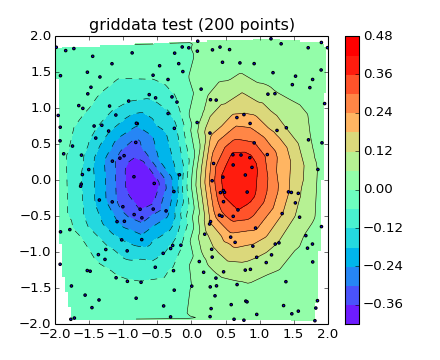
\includegraphics[width=4cm]{example_3.png} &
        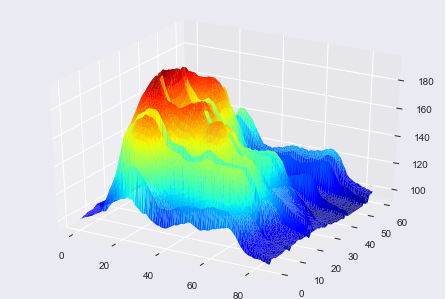
\includegraphics[width=4cm]{example_2.png}   \\
        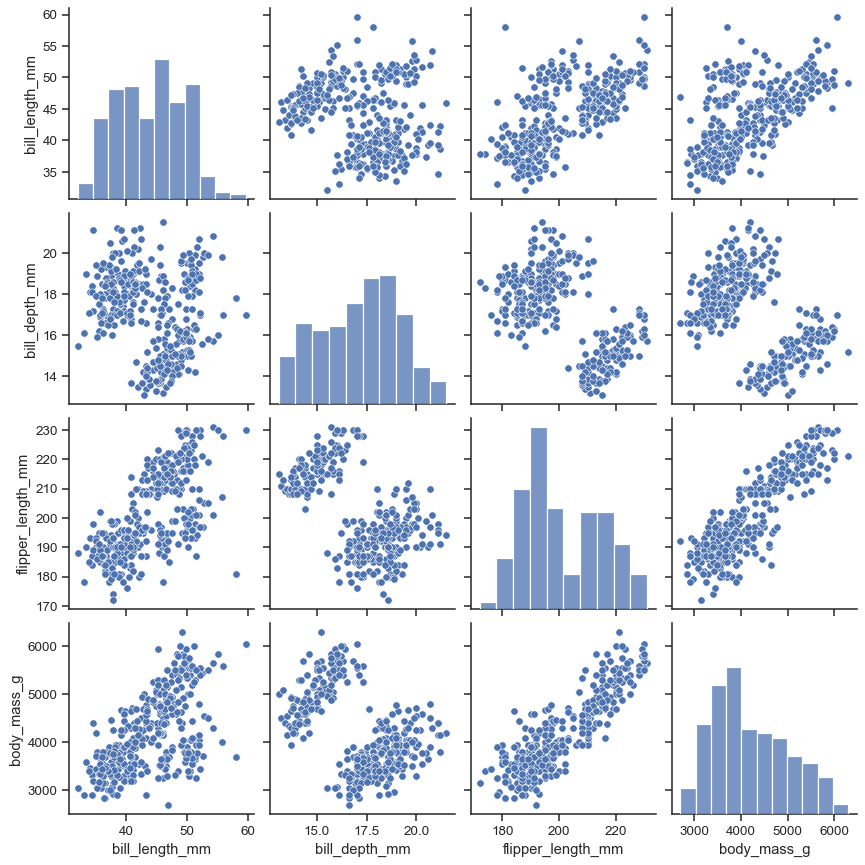
\includegraphics[width=4cm]{pairplot.png} &
        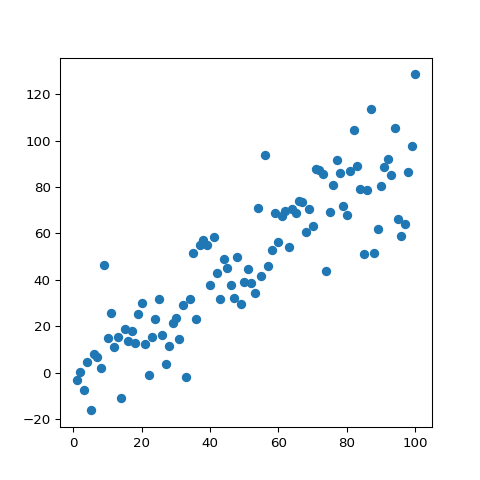
\includegraphics[width=4cm]{example_4.png}
    \end{tabular}
\end{frame}

\begin{frame}{Историческая справка}
    \begin{quote}
        The value of data visualization is not seeing “zillions” 
    of objects but rather recognizing relations among them.
    \rightline{Alfred Inselberg}
    \end{quote}
    \vspace{30px}
    \begin{itemize}
        \item Параллельные координаты были известны еще в 19-ом веке
        \item В 1980-ых были популяризированы Альфредом Инсельбергом
    \end{itemize}
\end{frame}

\begin{frame}{Классический график в параллельных осях}
    
    \vspace{10pt}

    \begin{itemize}
        \item Каждая линия соответствует объекту
        \item Каждая ось соответствует некоторой координате в пространстве
        \item Направление, порядок и масштаб осей может быть произвольным
    \end{itemize}

    \vspace{-5pt}

    \begin{figure}[htb]
        \centering
        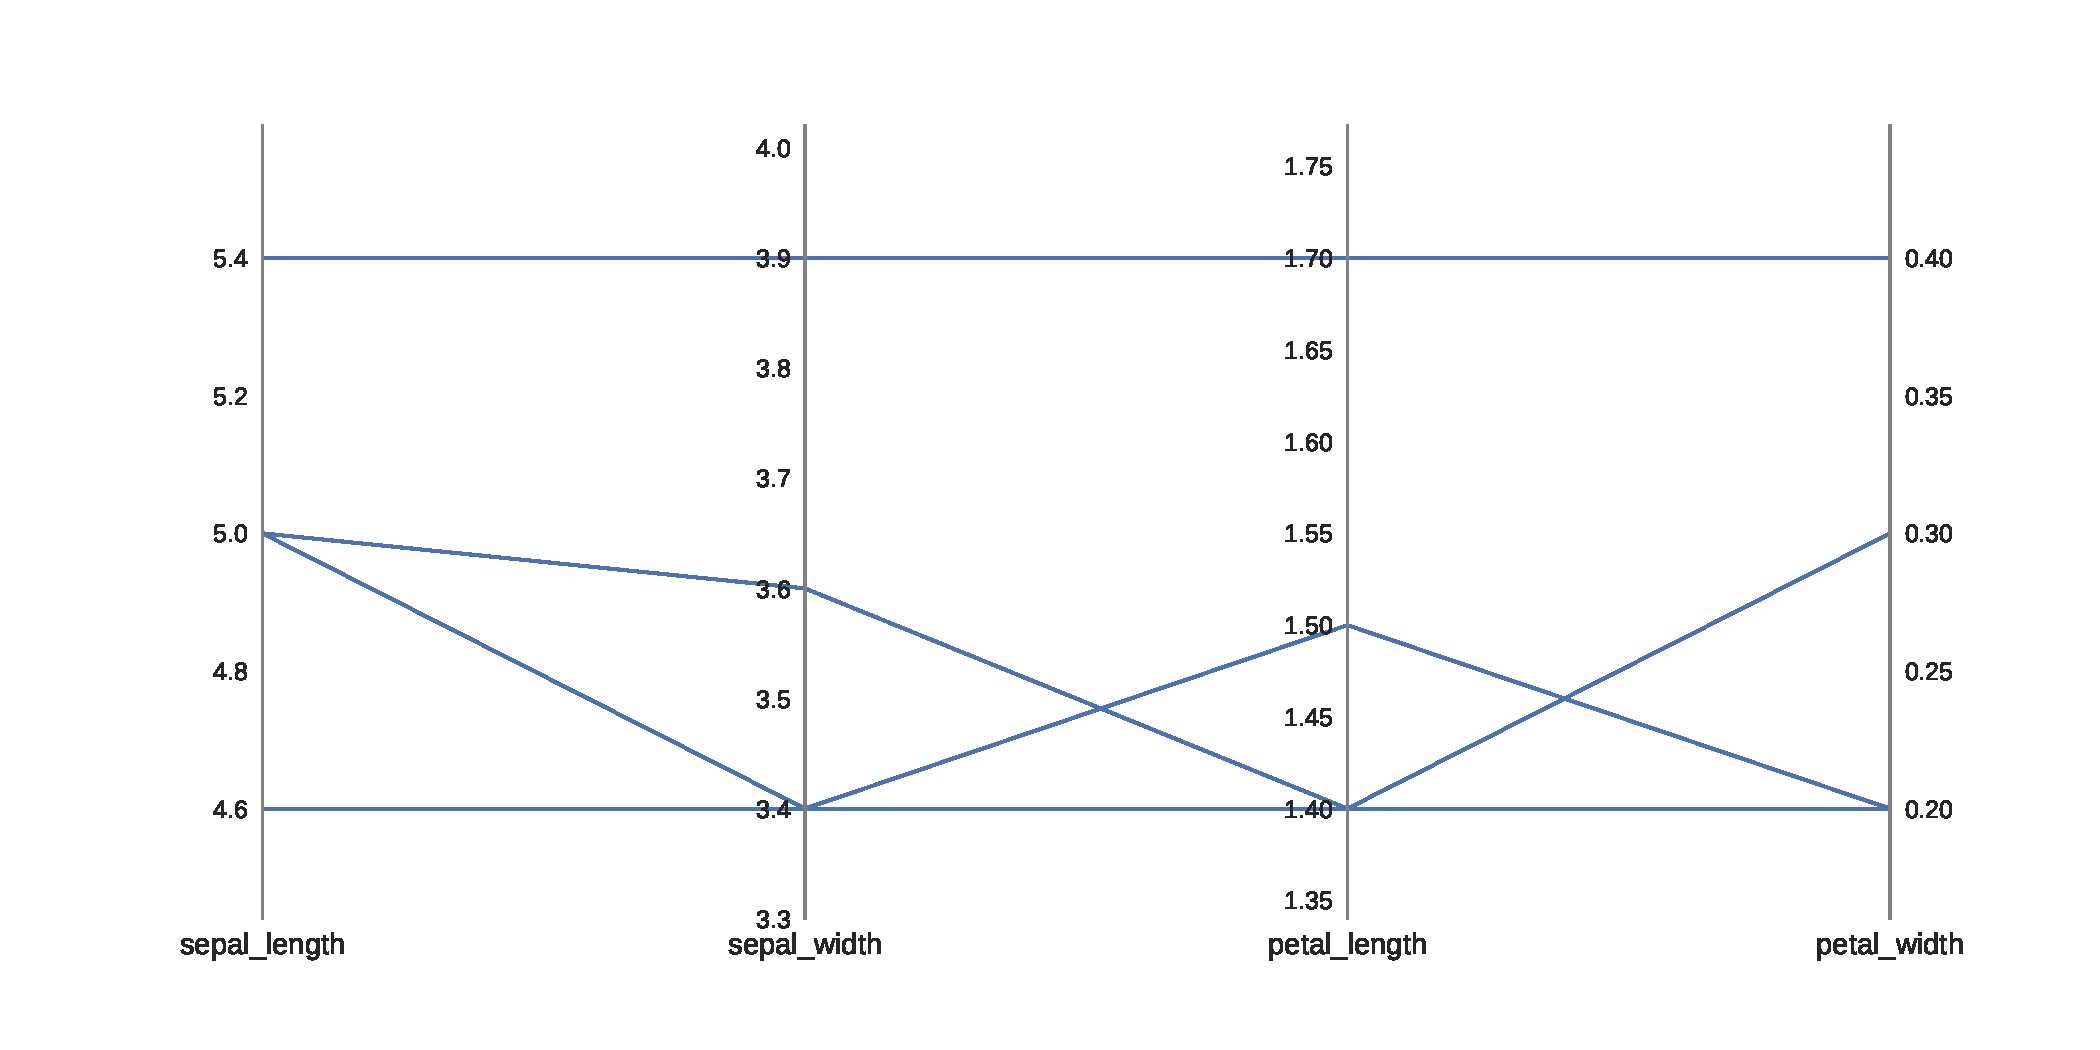
\includegraphics[width=10.5cm]{classic_pc.pdf}
    \end{figure}

\end{frame}

\section{Модификации}

\begin{frame}{Модификации: кластеры}

    \vspace{10px}

    Кластер — класс родственных элементов статистической совокупности.

    \begin{figure}[htb]
        \centering
        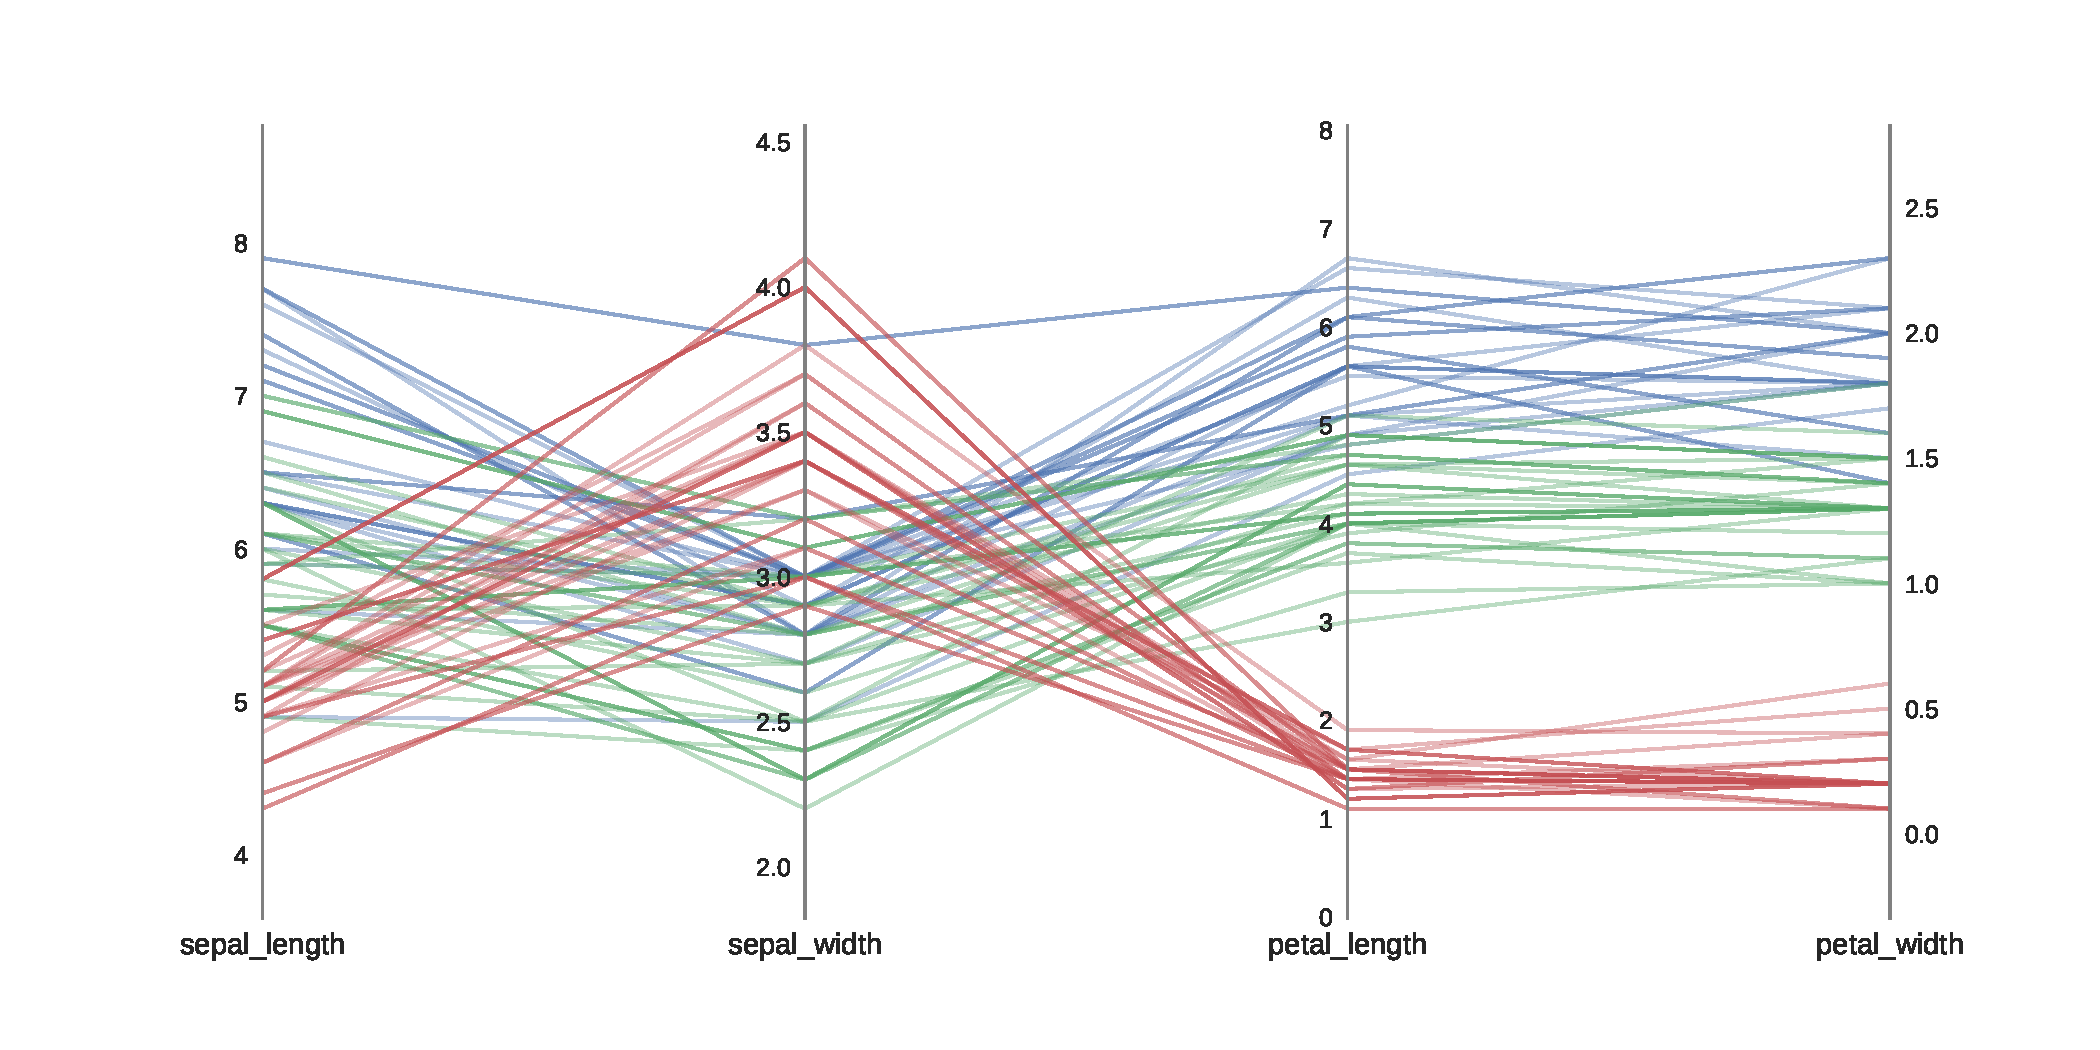
\includegraphics[width=10.5cm]{color_pc.pdf}
    \end{figure}

    Чаще всего именно в таком виде используют график в параллельных осях.
\end{frame}

\begin{frame}{Cглаживание линий}

    \vspace{10px}

    Человеку проще воспринимать гладкие линии, поэтому читаемость графика заметно возрастает.

    \begin{figure}[htb]
        \centering
        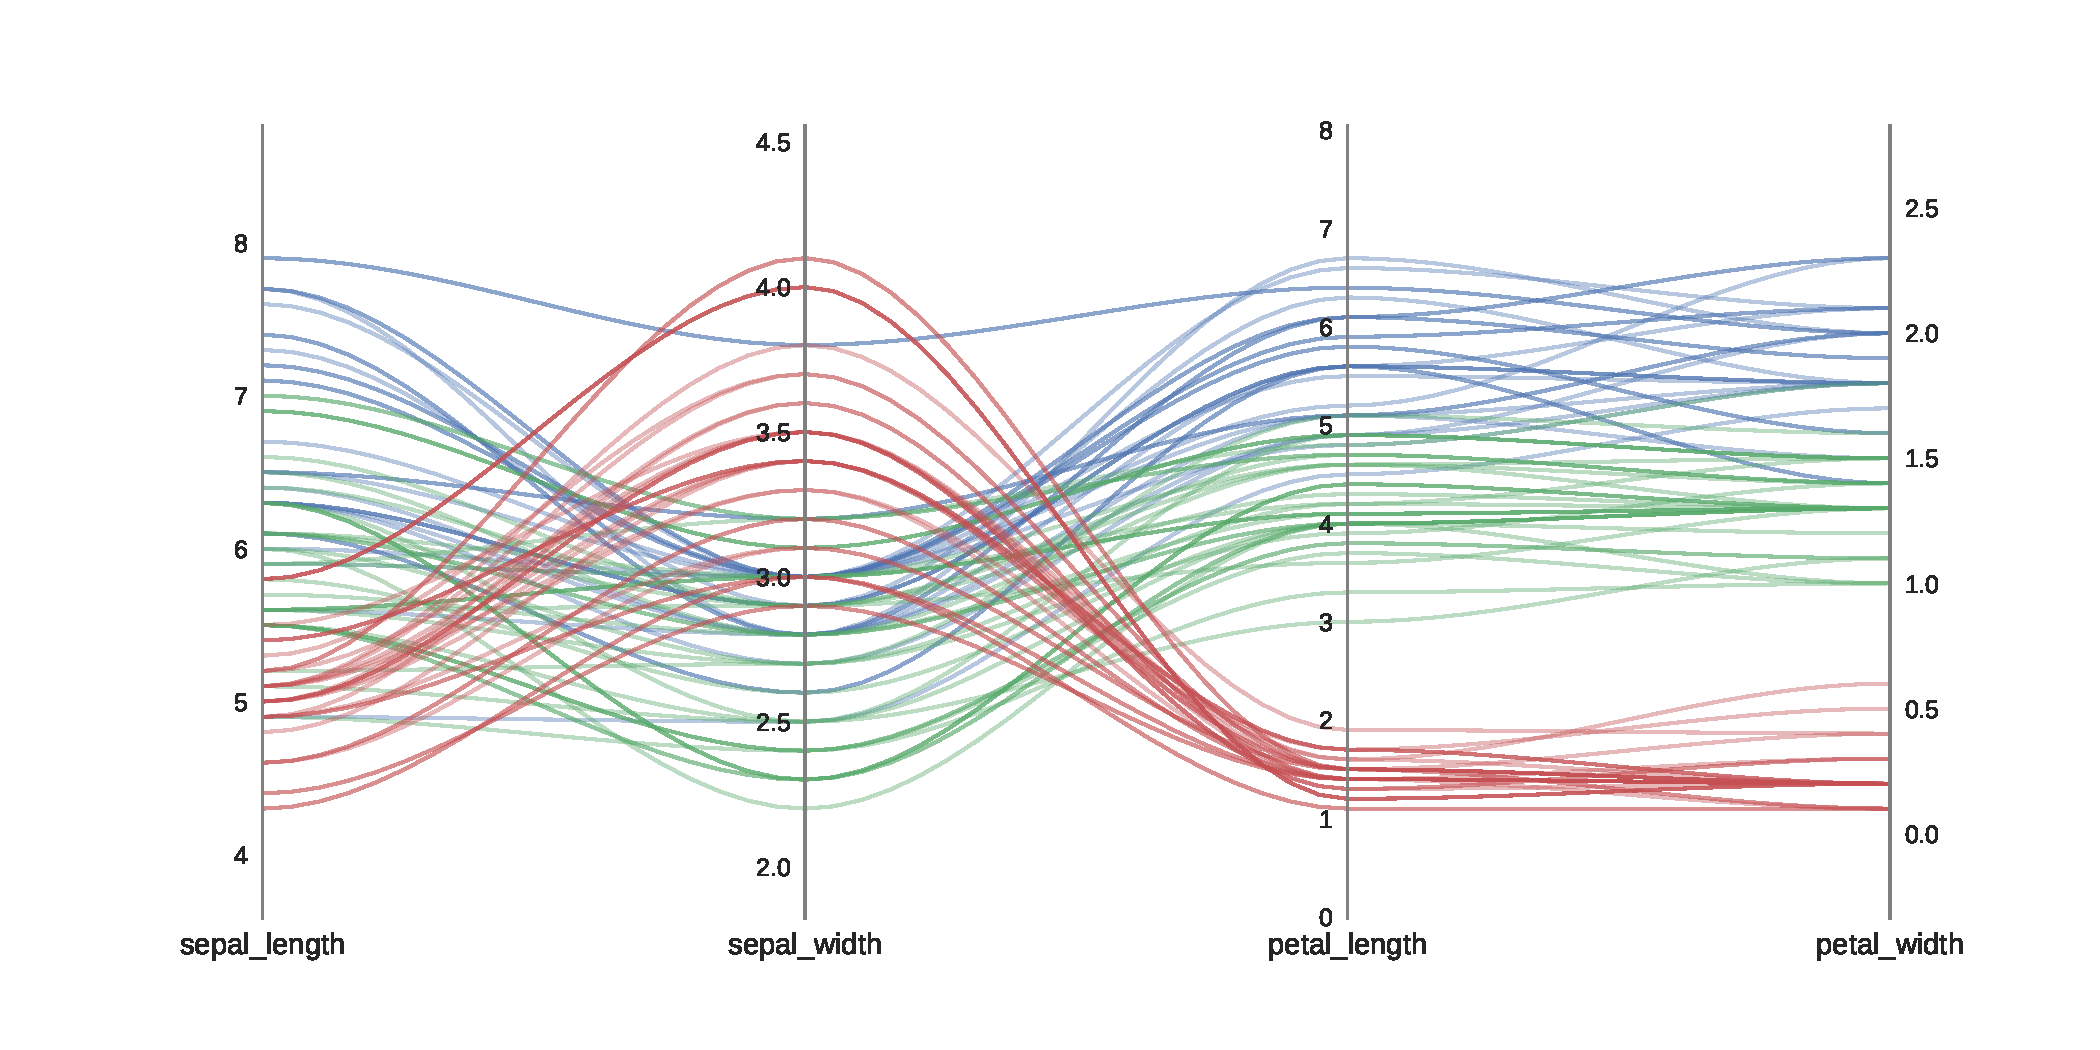
\includegraphics[width=10.5cm]{smooth_pc.pdf}
    \end{figure}
\end{frame}

\begin{frame}{Cвязывание линий}
    \begin{figure}[htb]
        \centering
        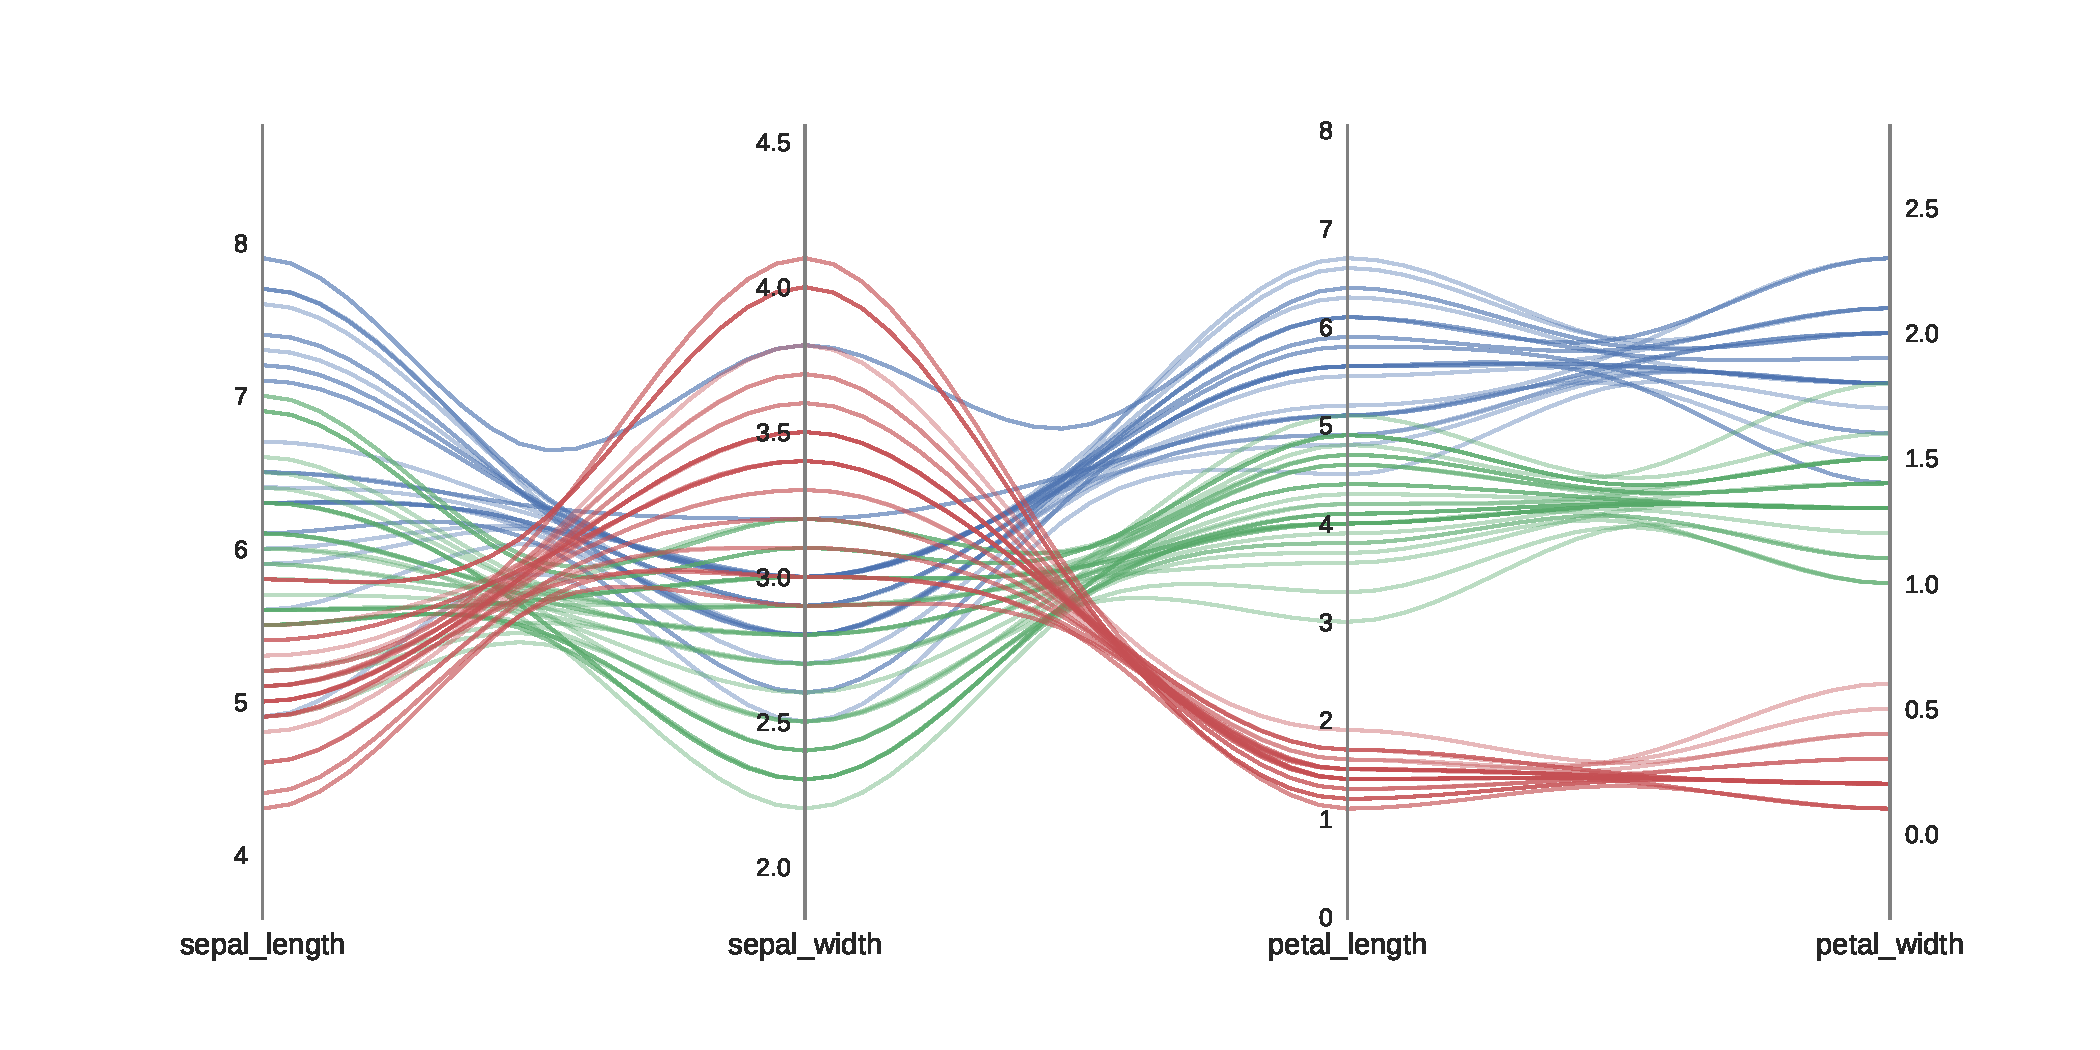
\includegraphics[width=10.5cm]{bundle_0.3_pc.pdf}
    \end{figure}
\end{frame}

\begin{frame}{Cвязывание линий}  
    Сильное связывание приводит к потере читаемости в рамках конкретного объекта,
    но увеличивает читаемость в рамках кластеров

    \begin{figure}[htb]
        \centering
        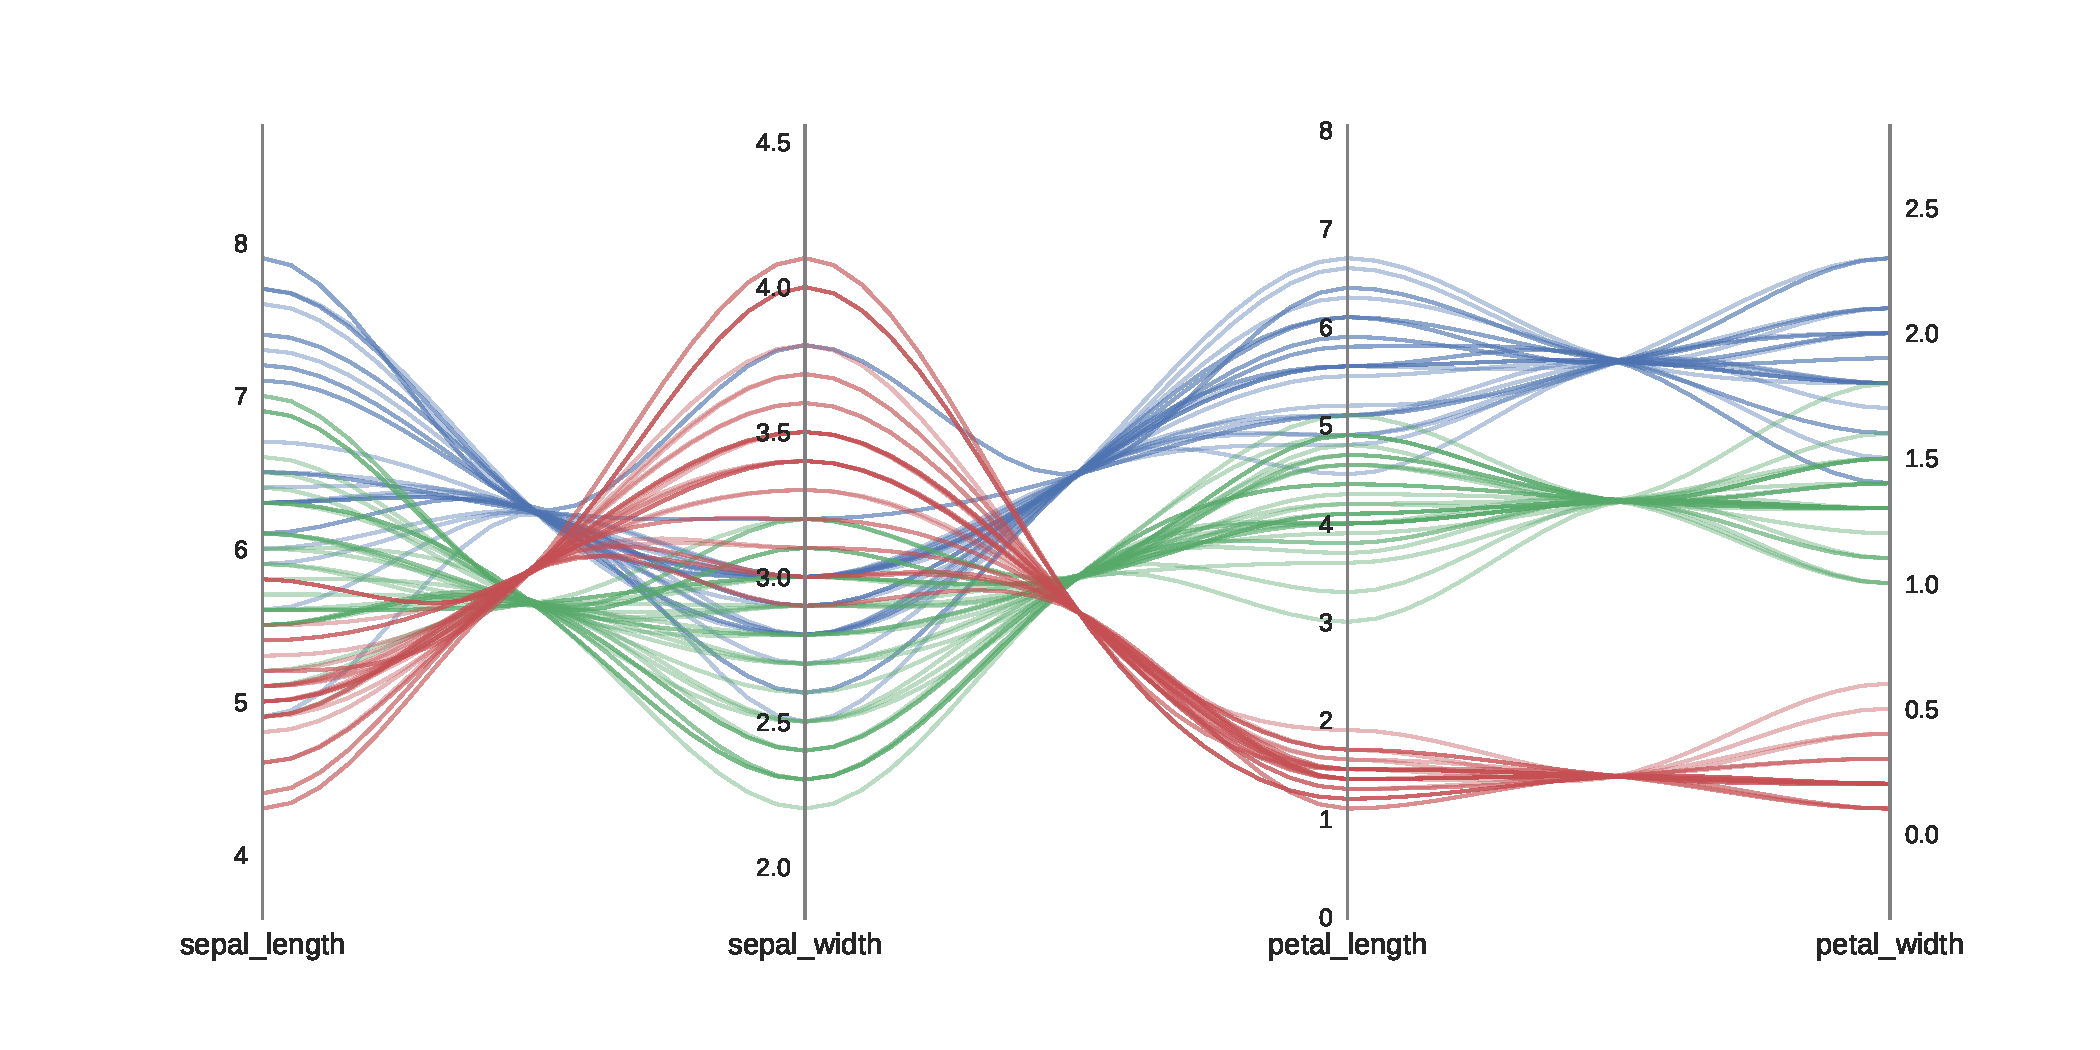
\includegraphics[width=10.5cm]{bundle_0.01_pc.pdf}
    \end{figure}
\end{frame}

\begin{frame}{Иерархические графики}

    Изображаем статистики распределений соответствующих кластеров (std, min, max, mean)
    вместо отрисовки каждого объекта.

    \begin{figure}[htb]
        \centering
        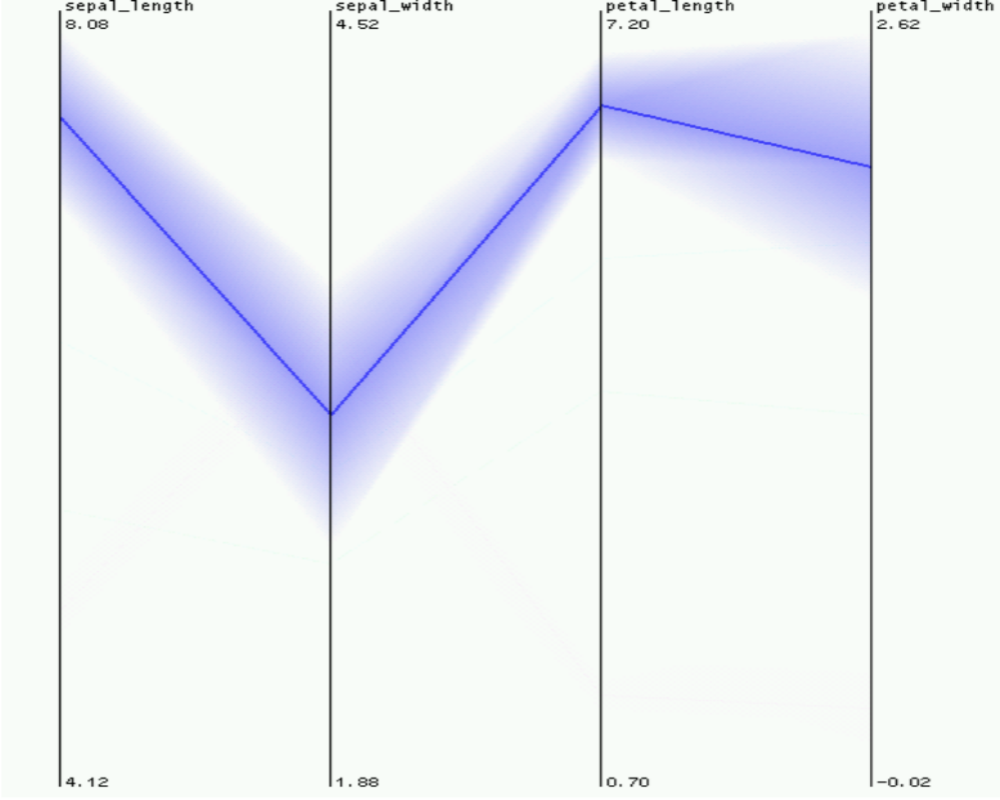
\includegraphics[width=5cm]{hierarchical_1.png}
    \end{figure}
\end{frame}

\begin{frame}{Иерархические графики}
    Пусть $X=(x_1,\ldots,x_n)$ -- выборка, где $x_i\in \mathbb{R}^n$. 

    \vspace{10px}

    Назовем множество $P$ m-разбиением множества X на m-подмножеств $\{P_1,\ldots,P_m\}$
    такое, что:
    \begin{align}
        \notag &1. P_i \cap  P_j = \oslash, \hspace{10px} \forall i,j =\overline{1,m} \\
        \notag &2. \bigcup\limits_{i=1}^{m} P_i = X 
    \end{align}

    Организуем иерархическую структуру в виде дерева, где корню соответствует $X$, 
    а каждая вершина сопоставлена элементу разбиения родительской вершины.

    \vspace{10pt}

    \textit{Синонимы: агломеративная кластеризация, иерархическая кластеризация}
\end{frame}

\begin{frame}{Пример иерархического разбиения}


    \begin{figure}[htb]
        \centering
        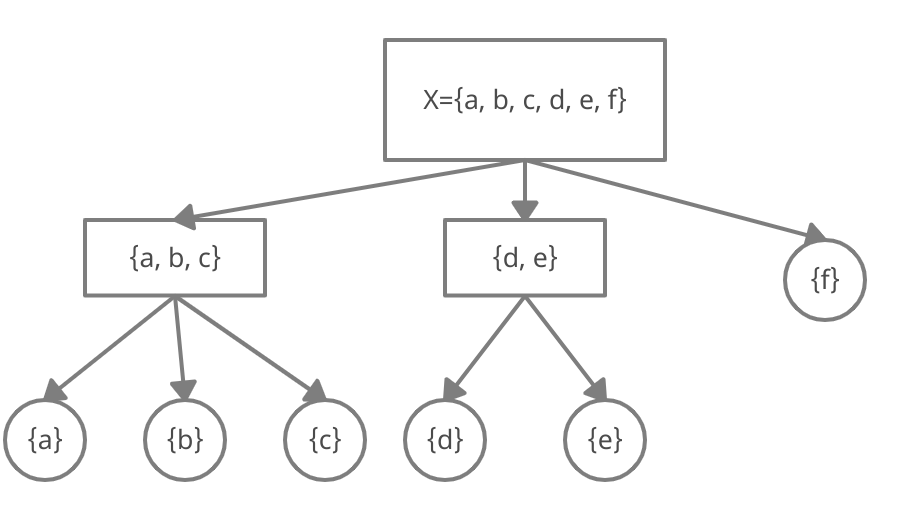
\includegraphics[width=10cm]{hierarchical_graph.png}
    \end{figure}
\end{frame}


\begin{frame}{Иерархические графики}

    \vspace{-20pt}

    Регулируя глубину, мы добавляем/уменьшаем количество кластеров на графике

    \vspace{20pt}

    \begin{tabular}{ccc}
        \centering
        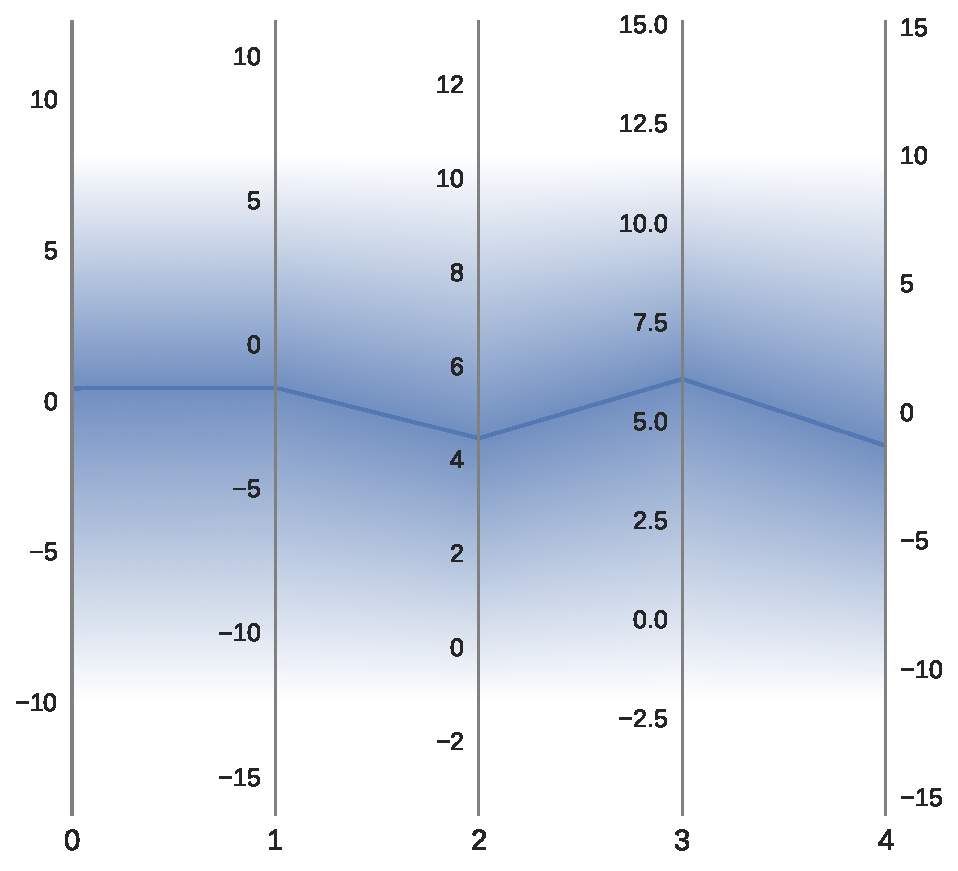
\includegraphics[width=3.2cm]{h_clustering_1.pdf} &
        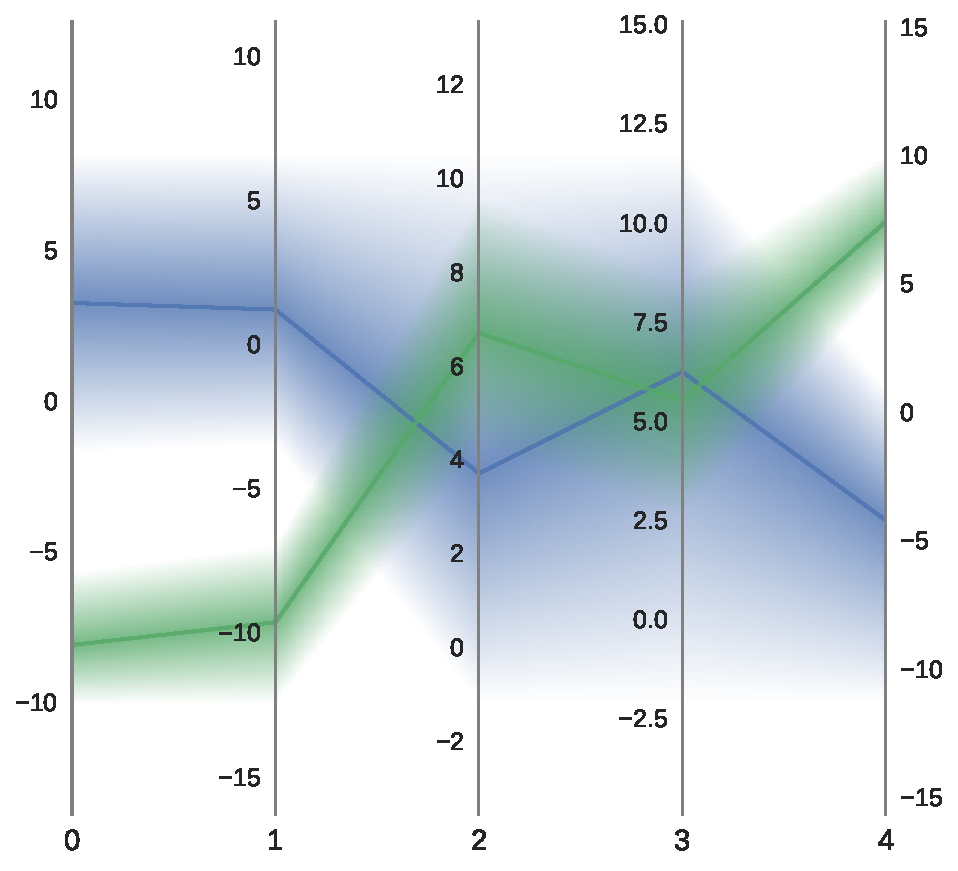
\includegraphics[width=3.2cm]{h_clustering_2.pdf} &
        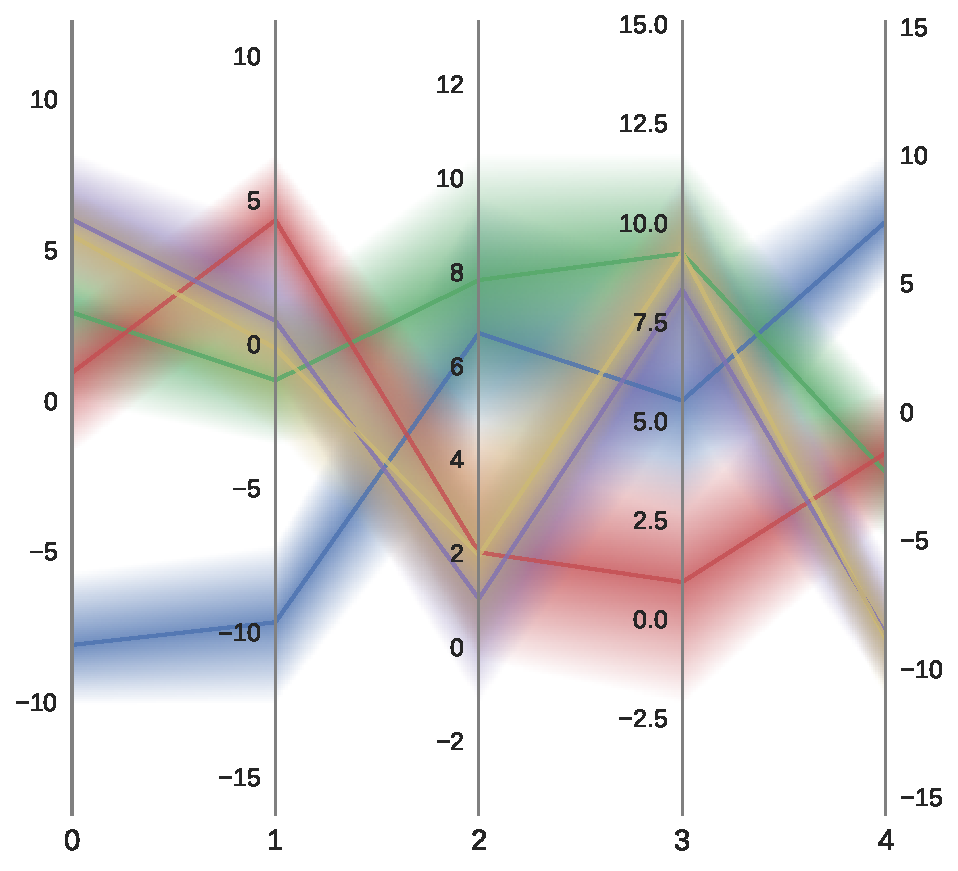
\includegraphics[width=3.2cm]{h_clustering_5.pdf}

    \end{tabular}

\end{frame}

\begin{frame}{3D}
    \begin{tabular}{cc}
        \centering
        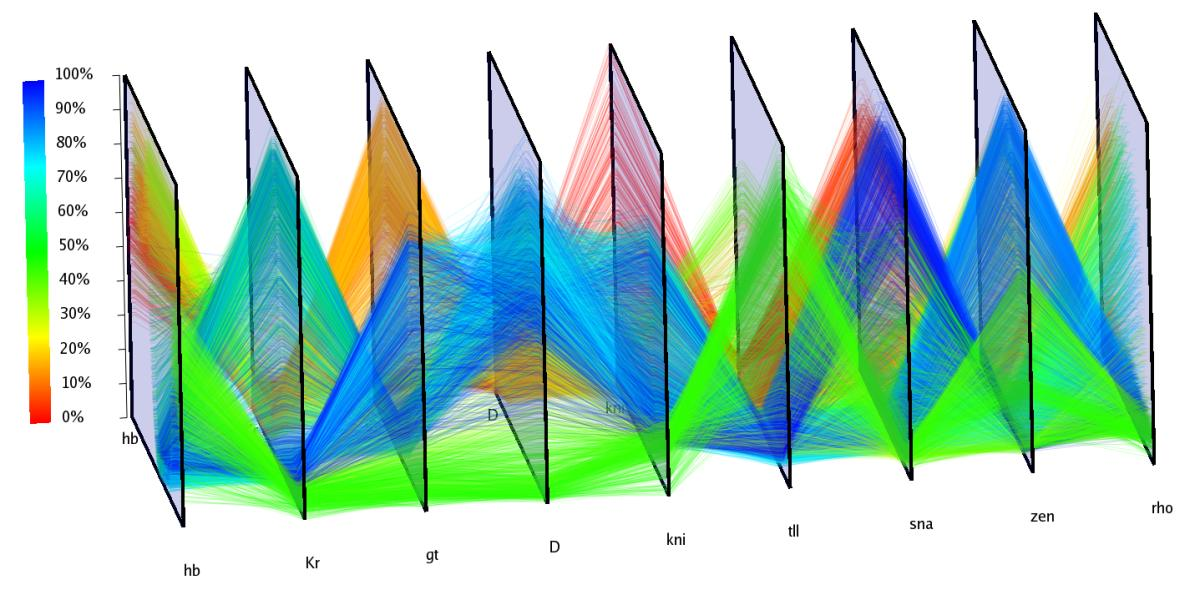
\includegraphics[width=6cm]{3d_pc.png} &
        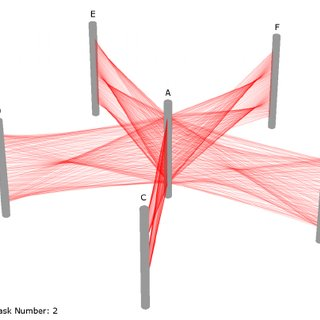
\includegraphics[width=3.5cm]{multi_relational_pc.png}   \\
        3D parallel coordinates & \makecell{3D multi-relational \\ parallel coordinates}
    \end{tabular}
\end{frame}


\section{Проблемы построения}

\begin{frame}{Плюсы и минусы}

    Плюсы:
    \begin{itemize}
        \item Решаем проблему визуализации многомерных пространств
        \item Высокая вариативность 
        \item Простая интерпретация
        \item Обнаружение аномалий (выбросов)
    \end{itemize}

    Минусы:
    \begin{itemize}
        \item Теряется читаемость на больших выборках
        \item Только вещественные признаки
        \item Много гиперпараметров
        \item Необходимость объяснять принцип построения графика
    \end{itemize}
\end{frame}


\begin{frame}{Естественные вопросы при построении}
    \begin{itemize}
        \item В каком порядке расположить оси?
        \item В какую сторону направлять оси?
        \item Как много объектов отобразить?
        \item Какой масштаб выбрать для каждой оси?
    \end{itemize}
\end{frame}

\begin{frame}{Выбор направлений и порядка осей}
    \begin{figure}[htb]
        \centering
        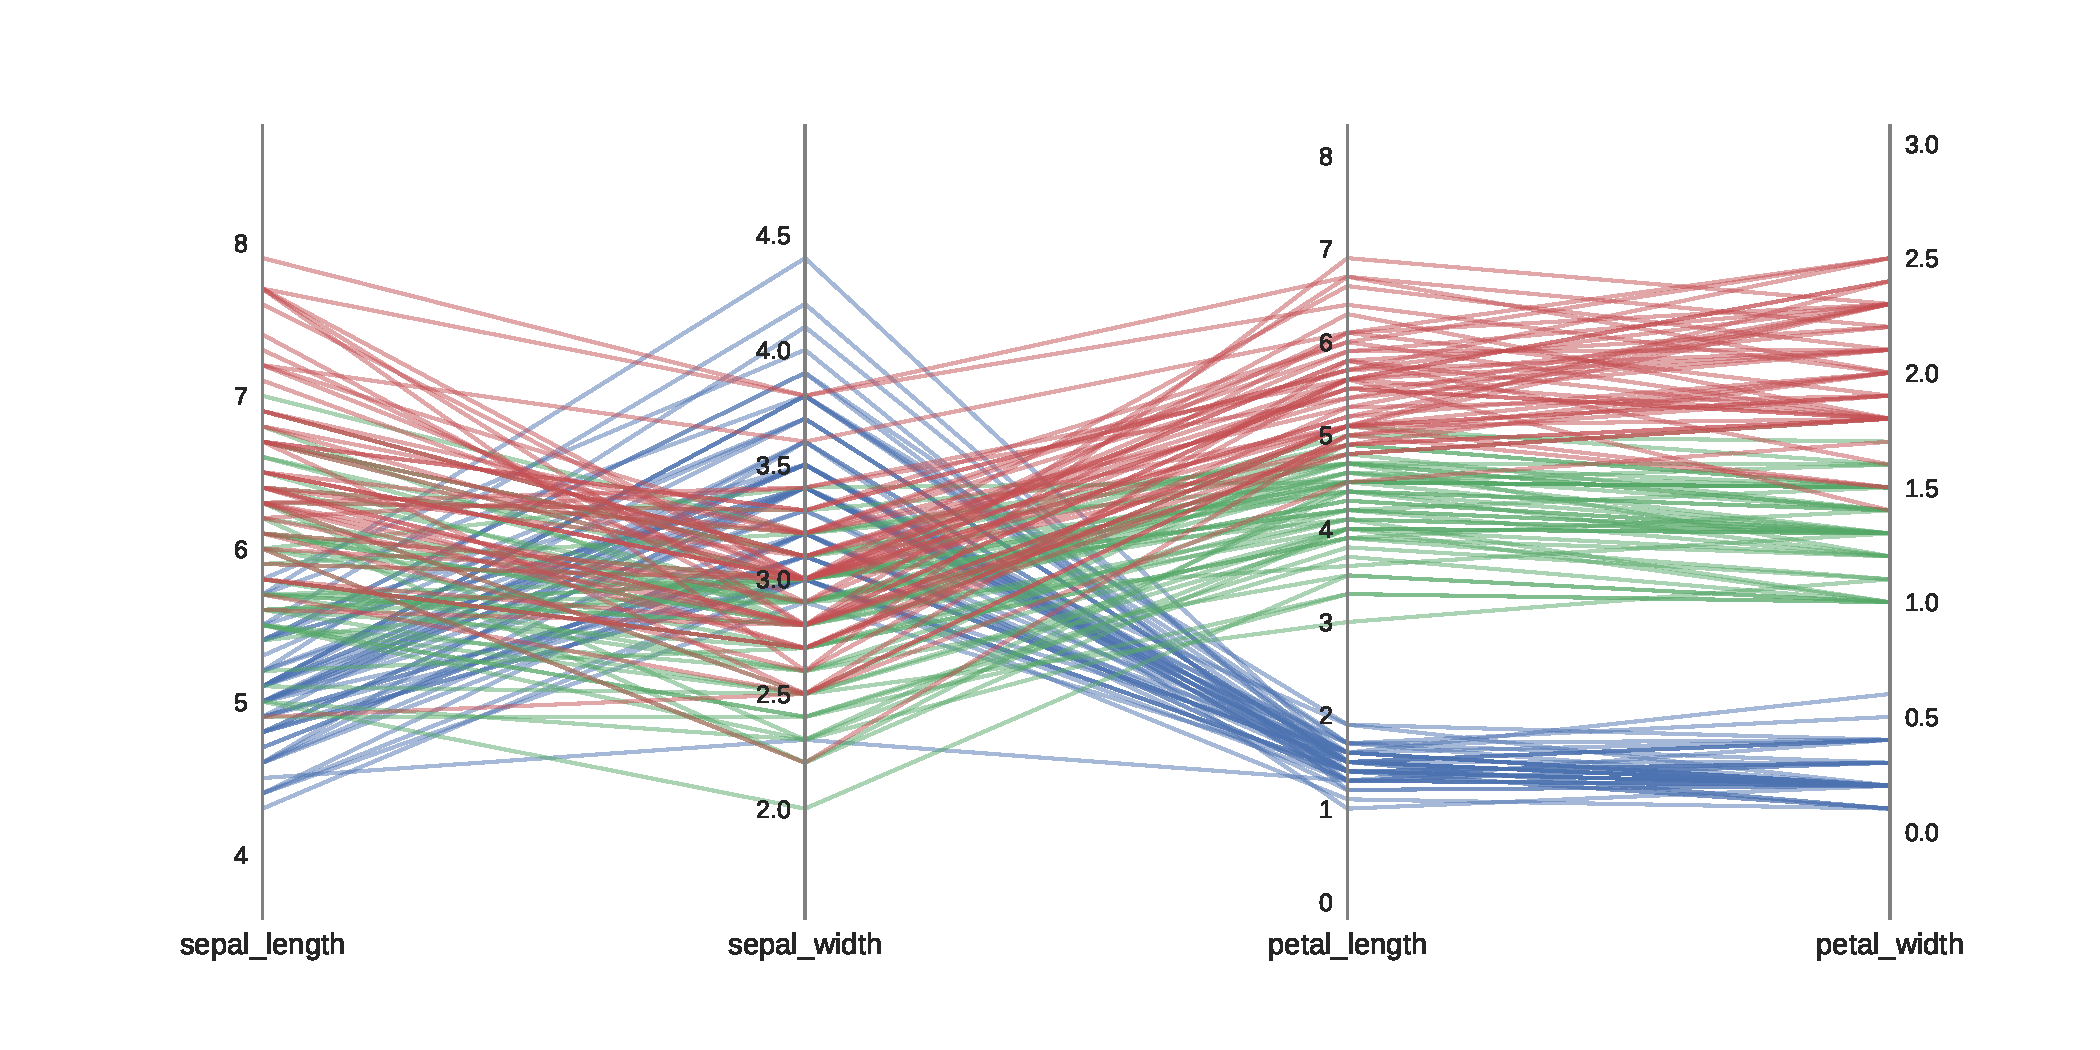
\includegraphics[width=10.5cm]{upgrade_1.pdf}
    \end{figure}
\end{frame}

\begin{frame}{Выбор направлений и порядка осей}
    \begin{figure}[htb]
        \centering
        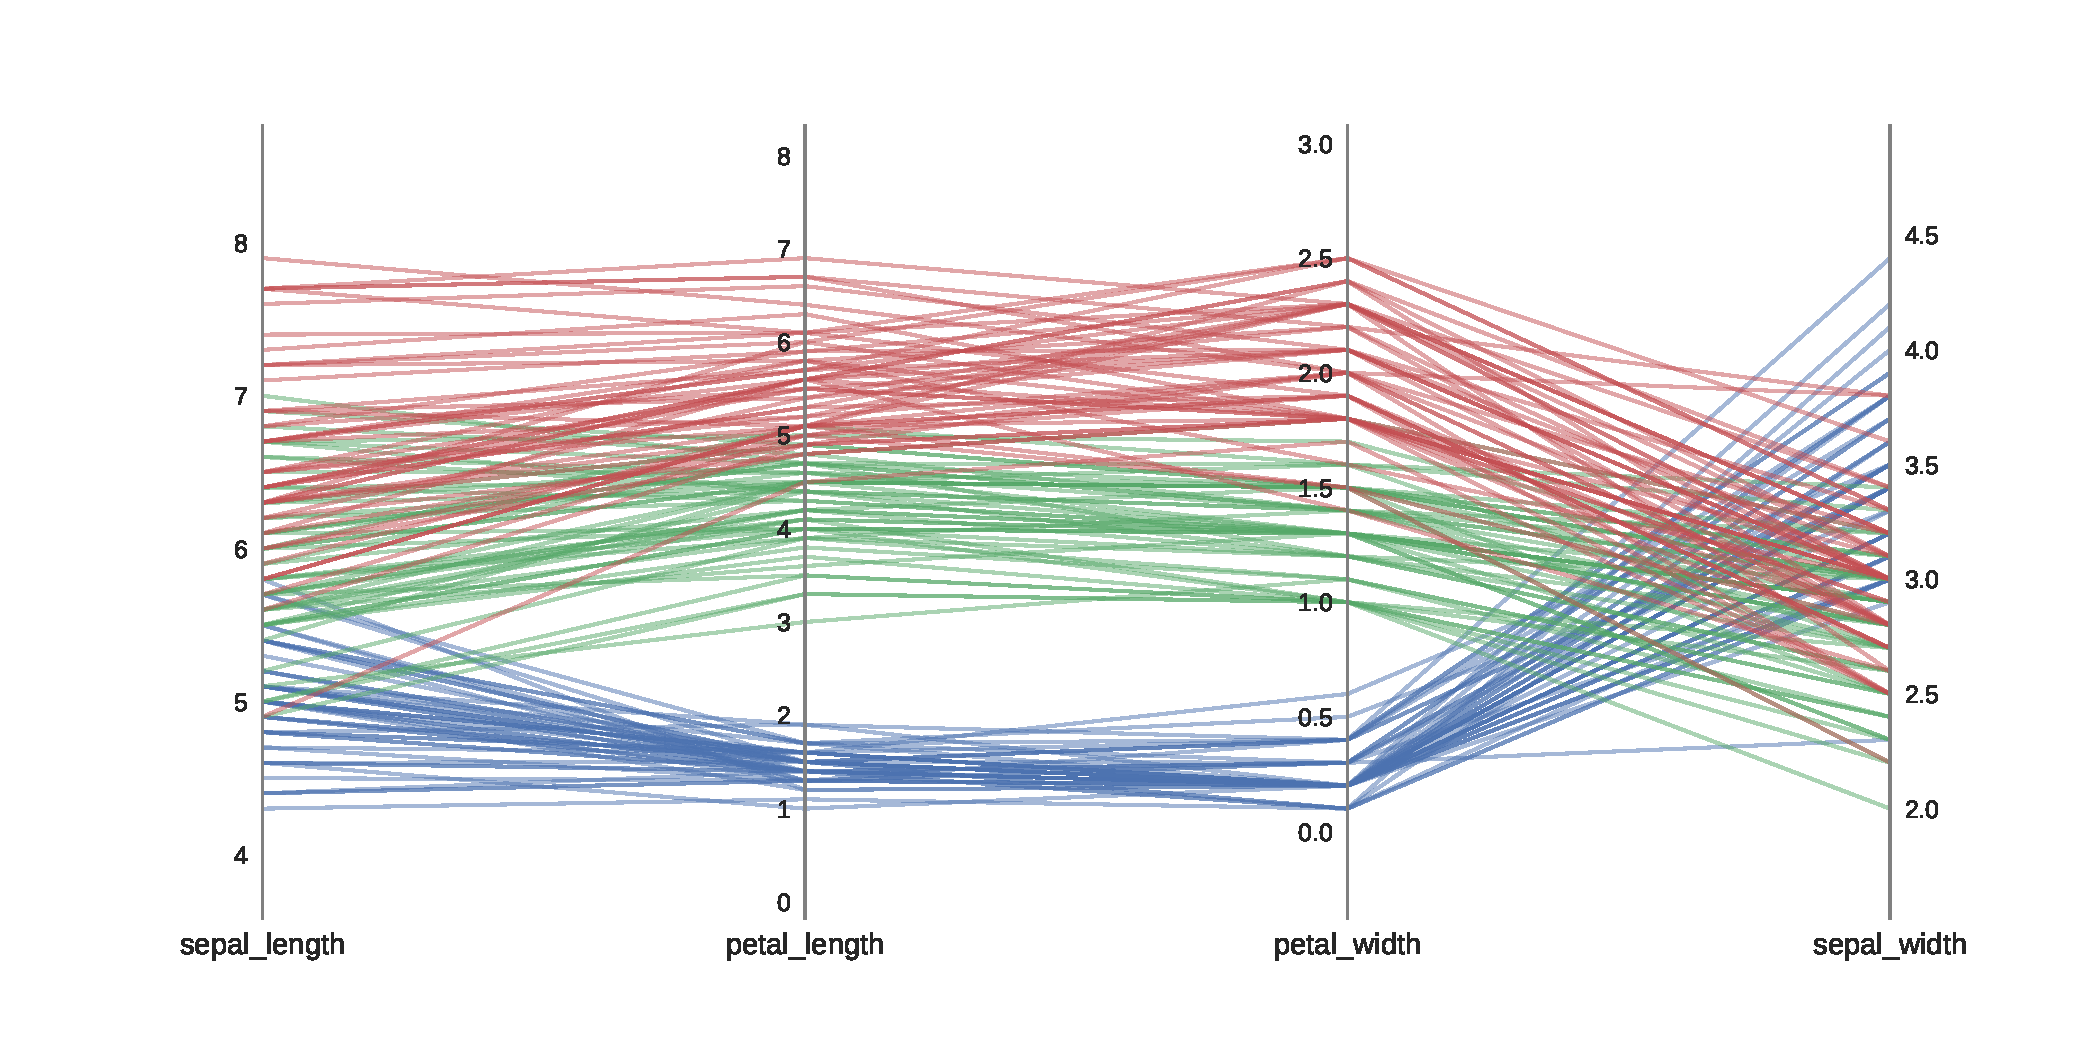
\includegraphics[width=10.5cm]{upgrade_2.pdf}
    \end{figure}
\end{frame}

\begin{frame}{Выбор направлений и порядка осей}
    \begin{figure}[htb]
        \centering
        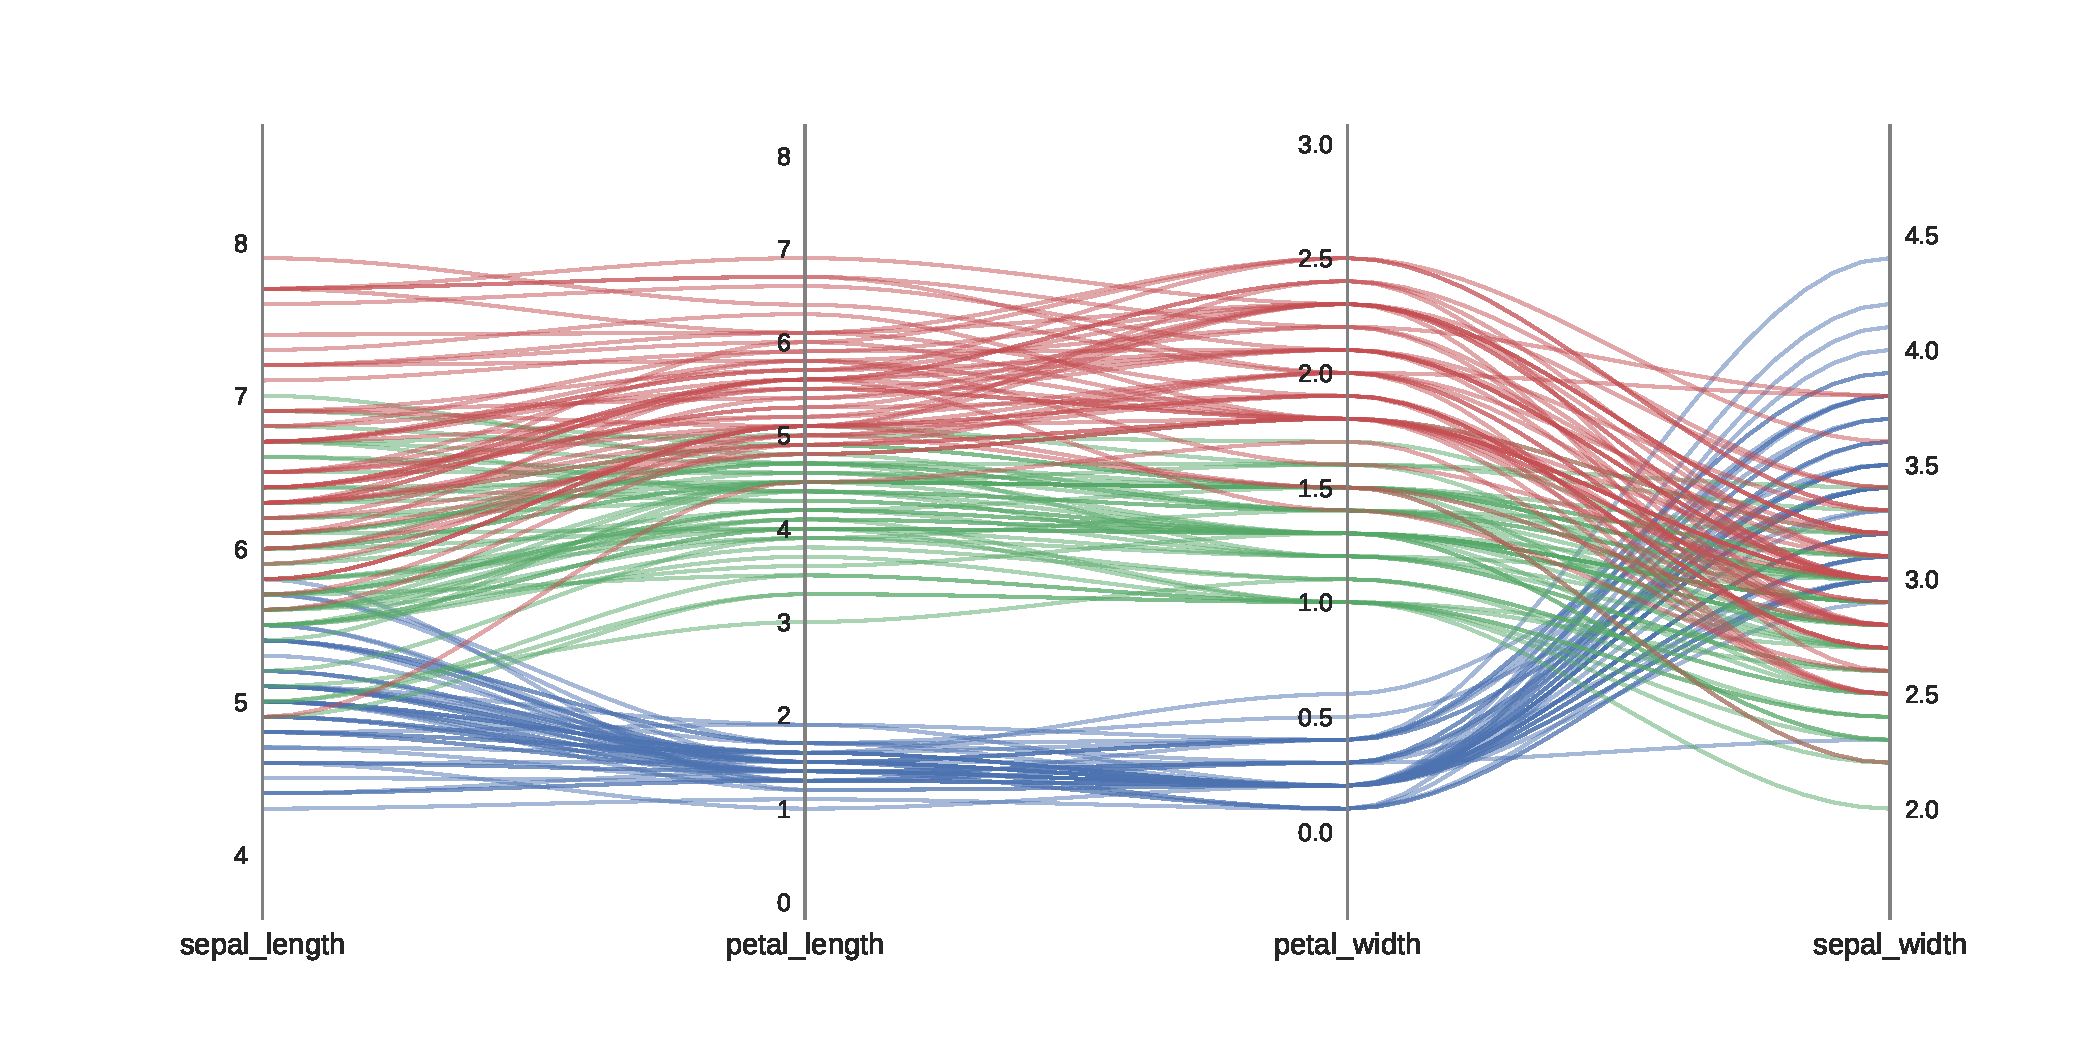
\includegraphics[width=10.5cm]{upgrade_3.pdf}
    \end{figure}
\end{frame}


\begin{frame}{Выбор направлений и порядка осей}
    \begin{figure}[htb]
        \centering
        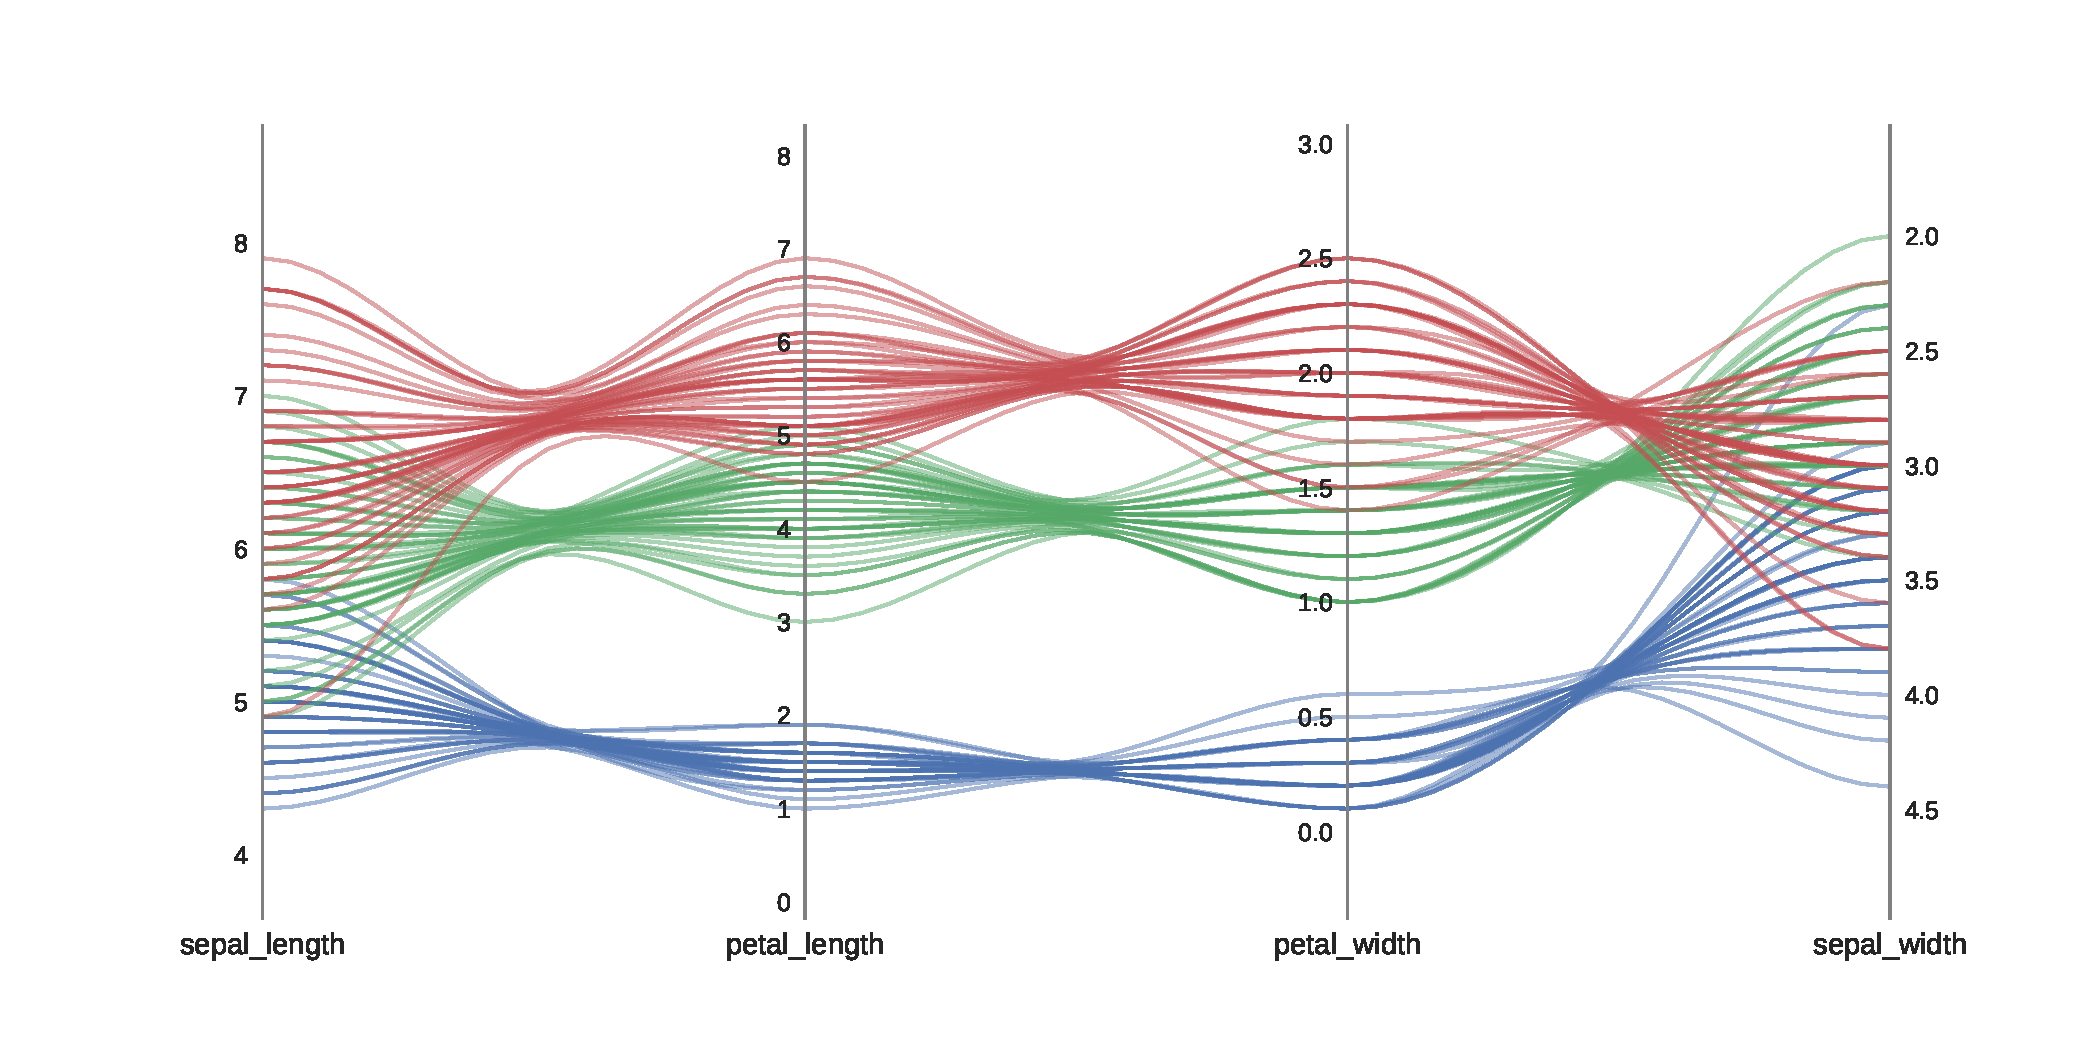
\includegraphics[width=10.5cm]{upgrade_4.pdf}
    \end{figure}
\end{frame}

\begin{frame}{Влияение количества объектов на читаемость}
    \begin{figure}[htb]
        \centering
        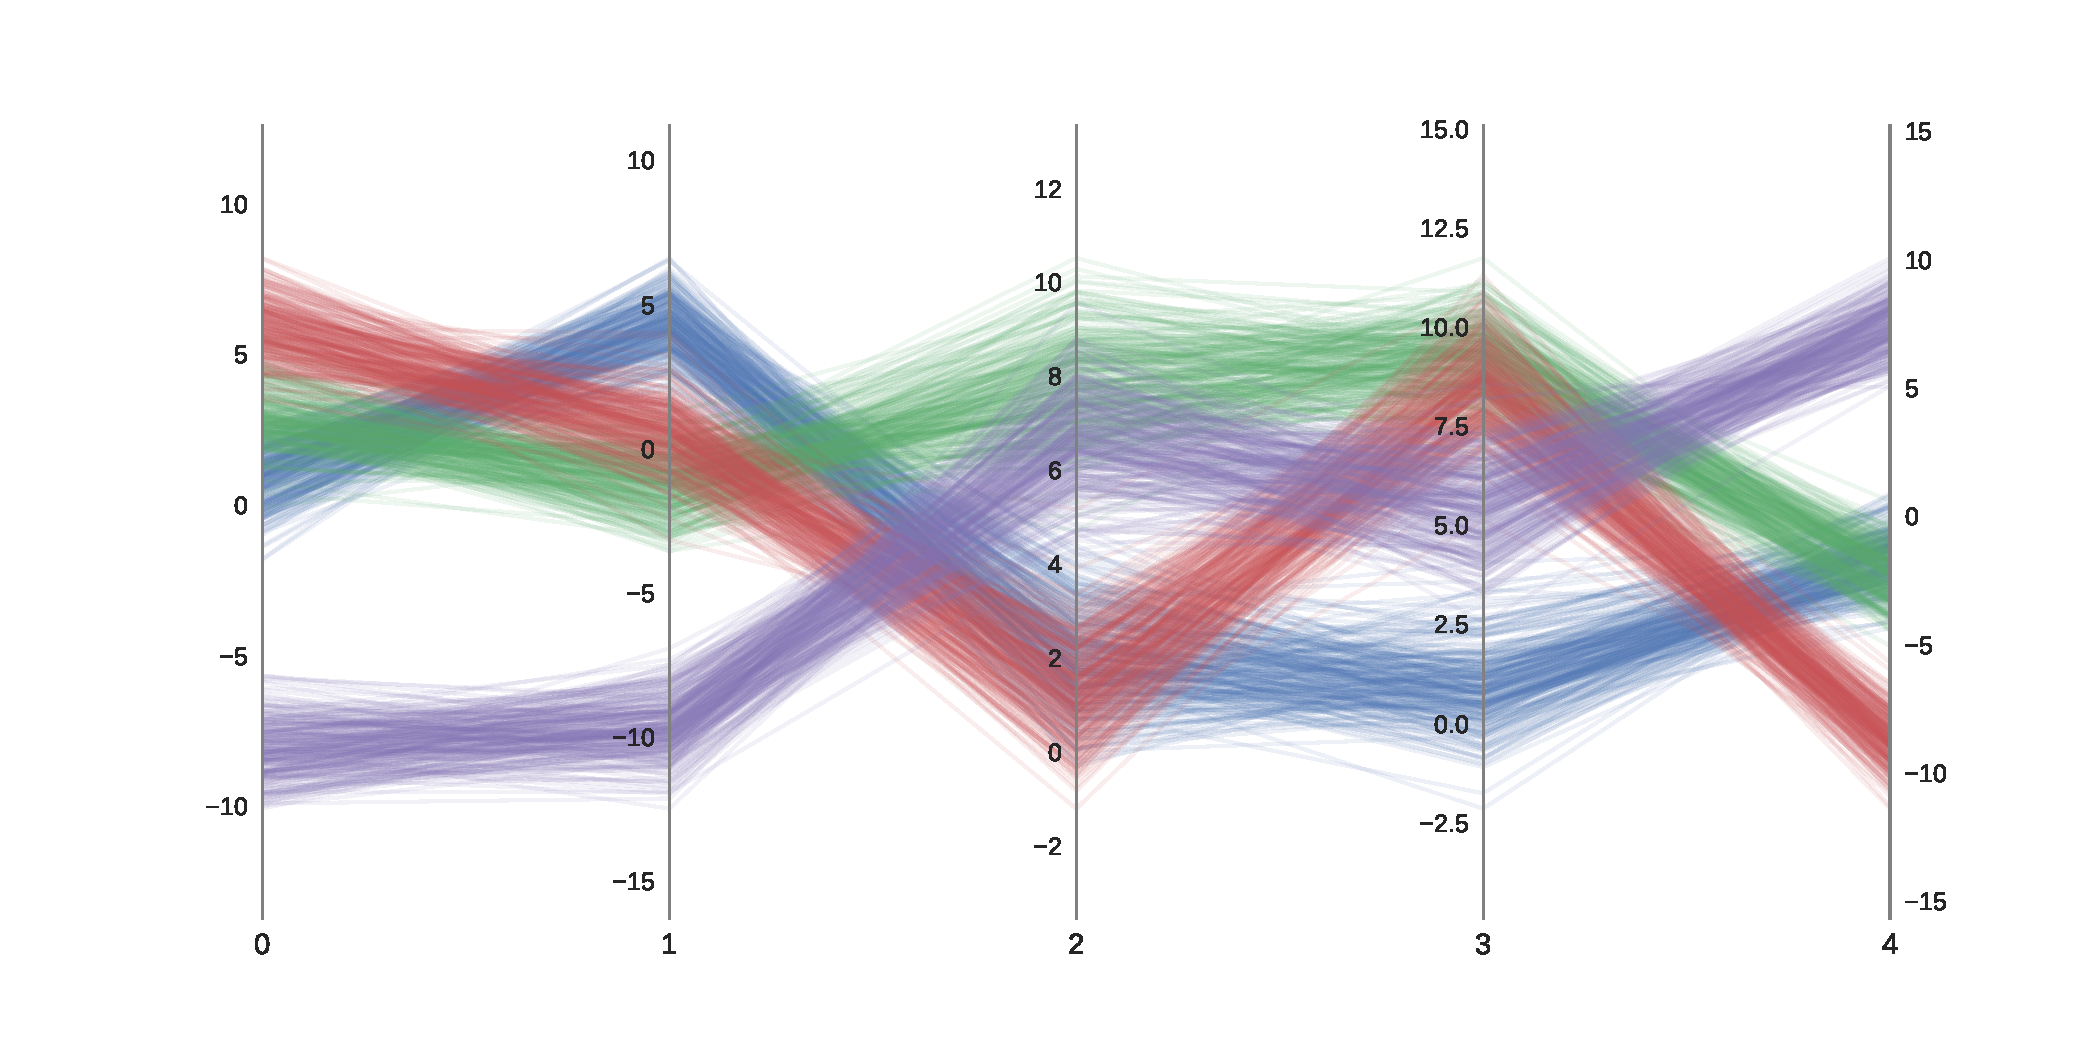
\includegraphics[width=10.5cm]{base_good_clustering.pdf}
    \end{figure}
\end{frame}

\begin{frame}{Влияение количества объектов на читаемость}
    \begin{figure}[htb]
        \centering
        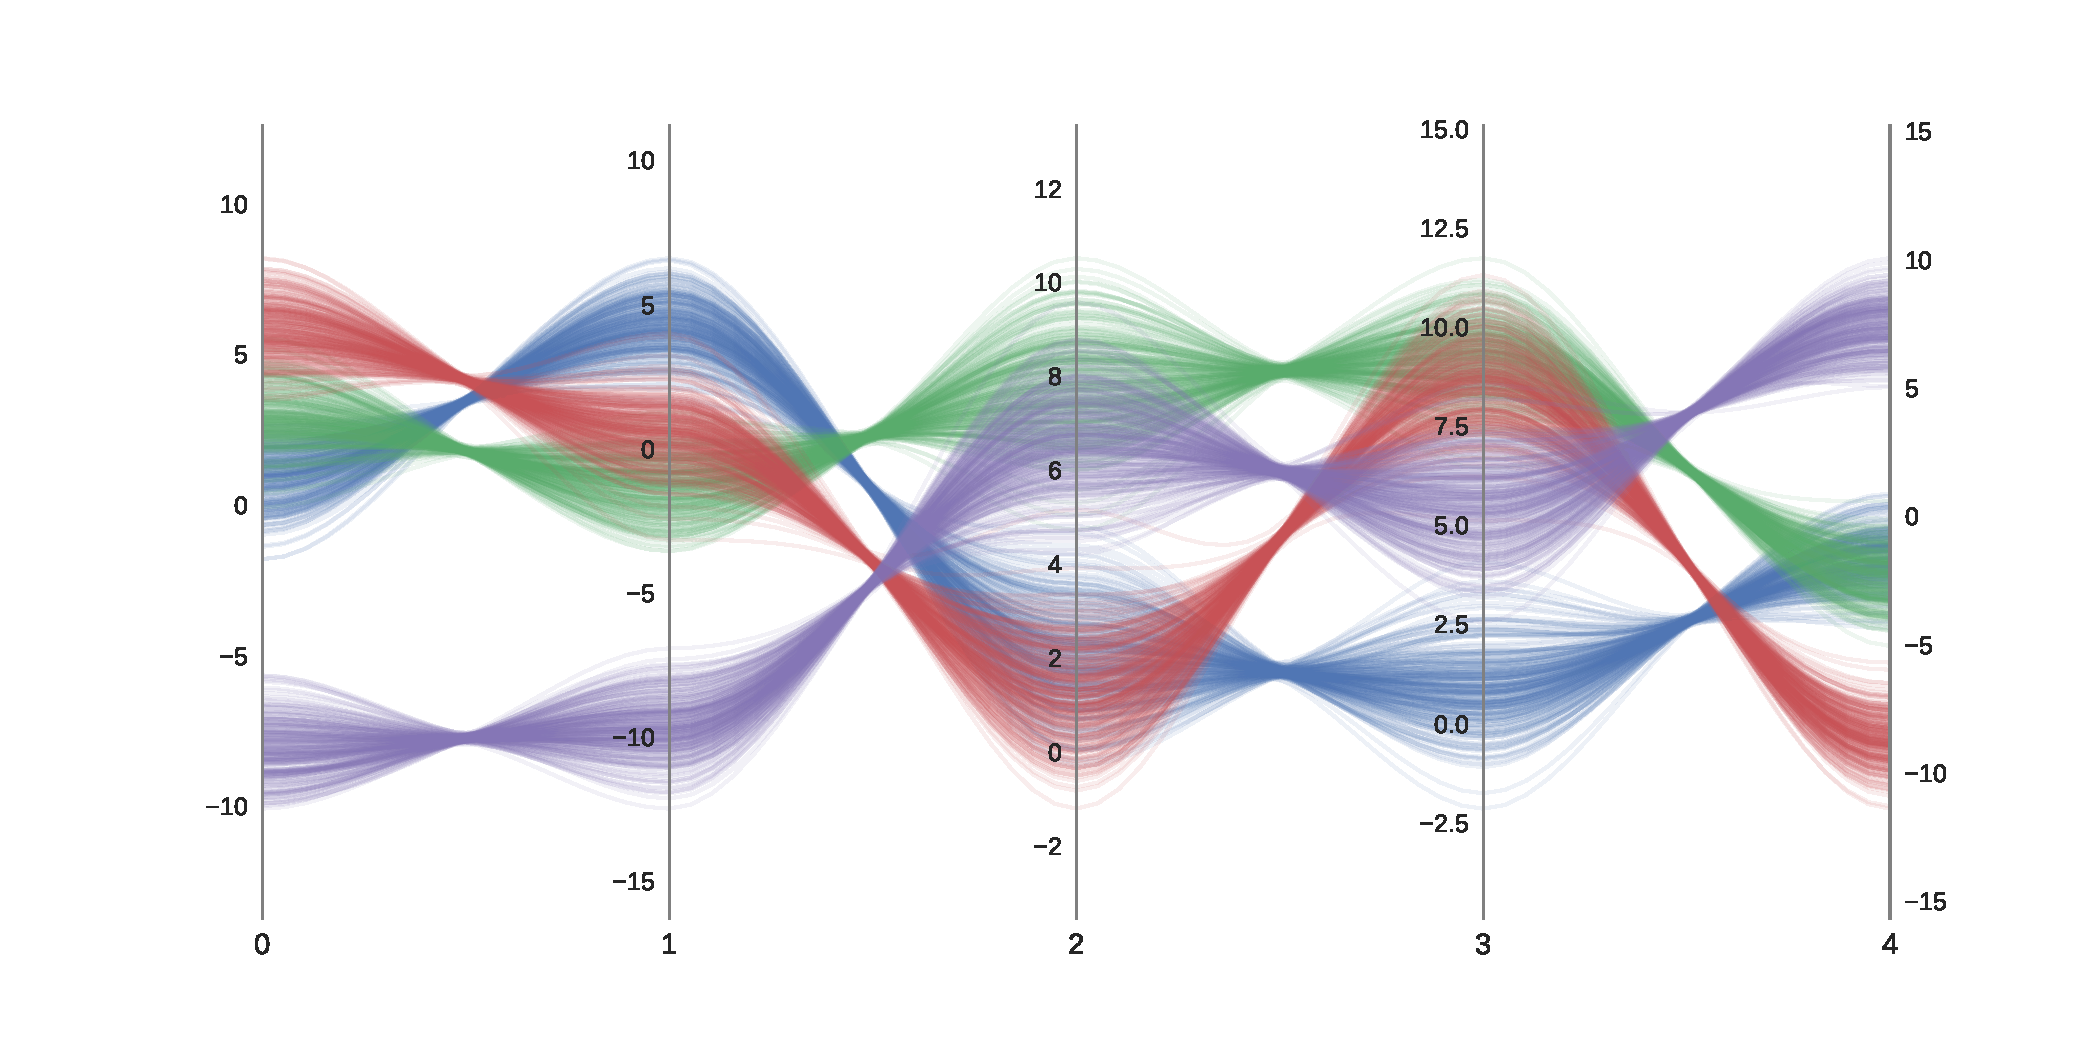
\includegraphics[width=10.5cm]{good_clustering.pdf}
    \end{figure}
\end{frame}

\begin{frame}{Влияение количества объектов на читаемость}
    \begin{figure}[htb]
        \centering
        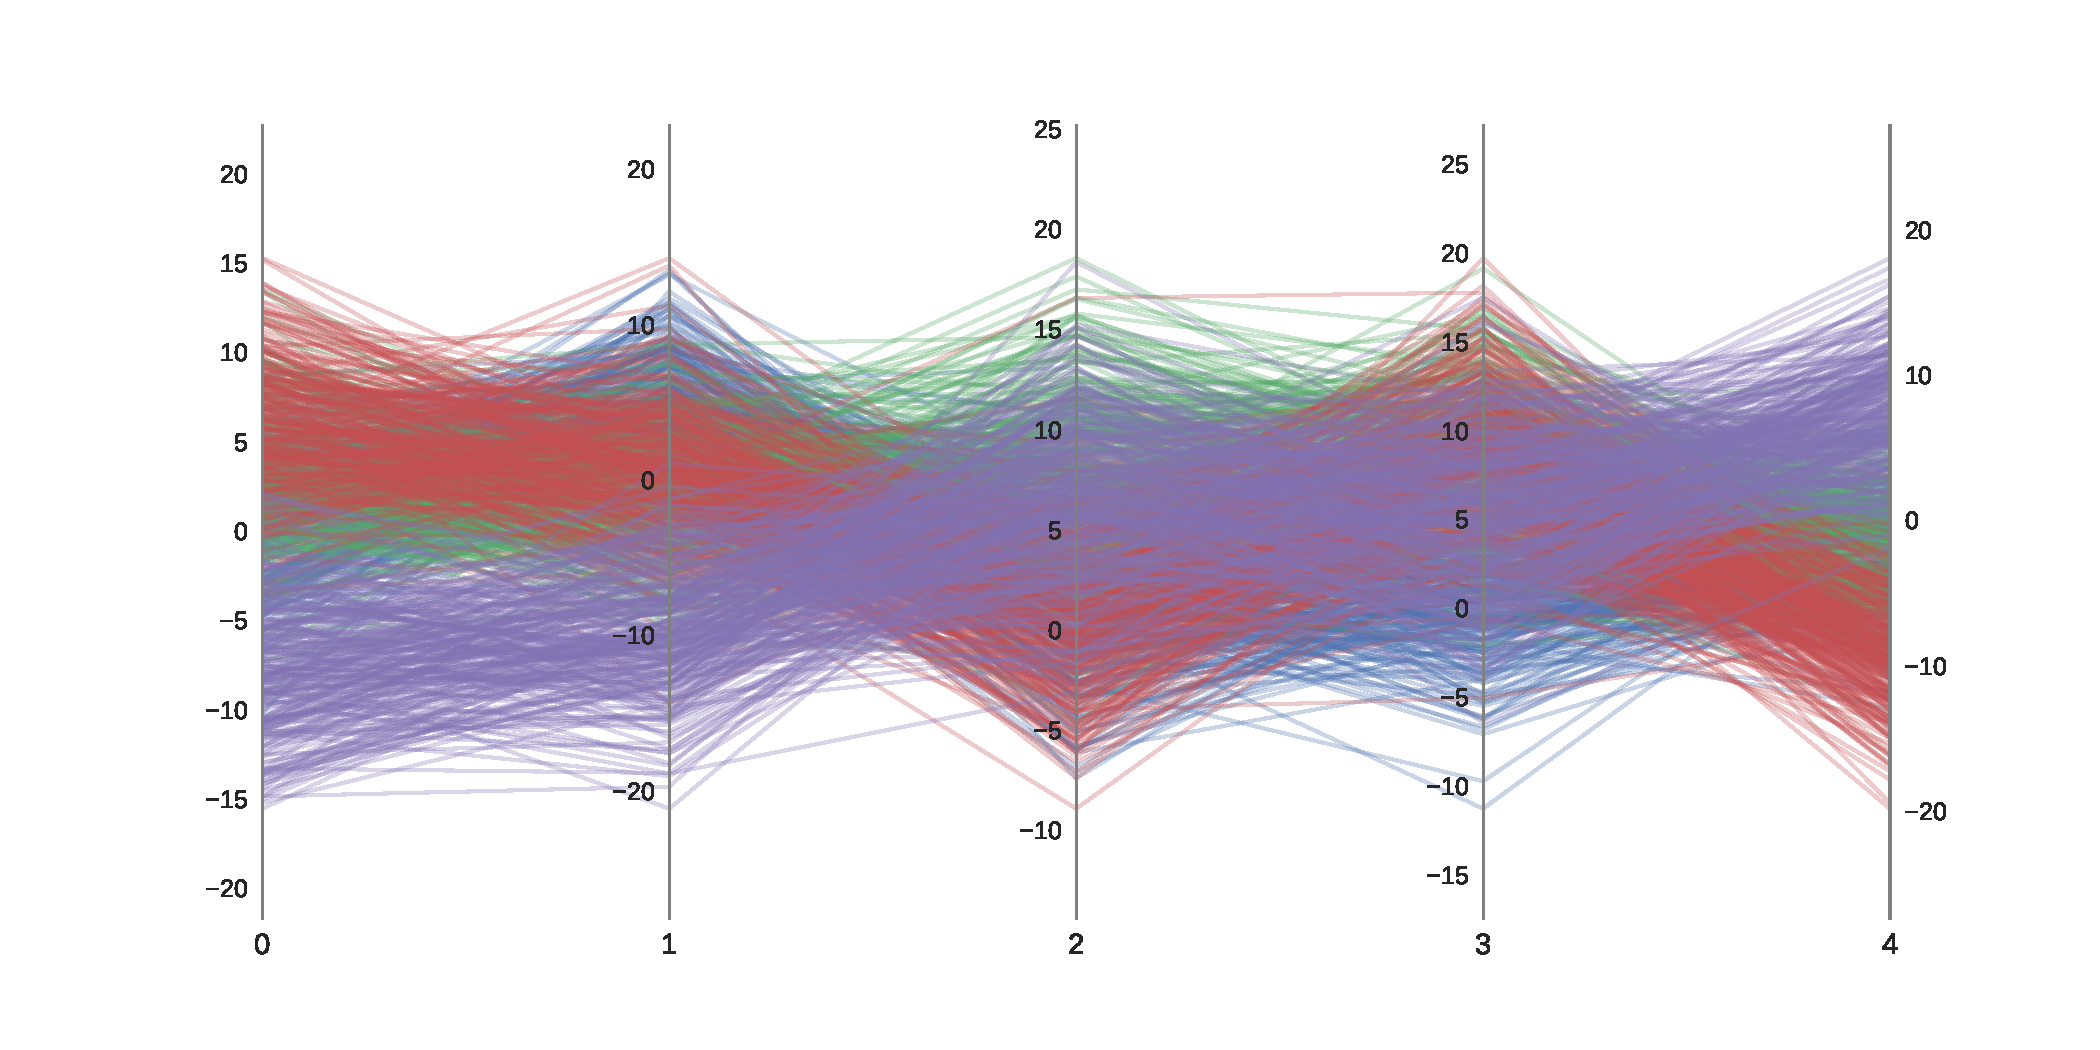
\includegraphics[width=10.5cm]{base_bad_clustering.pdf}
    \end{figure}
\end{frame}

\begin{frame}{Влияение количества объектов на читаемость}
    \begin{figure}[htb]
        \centering
        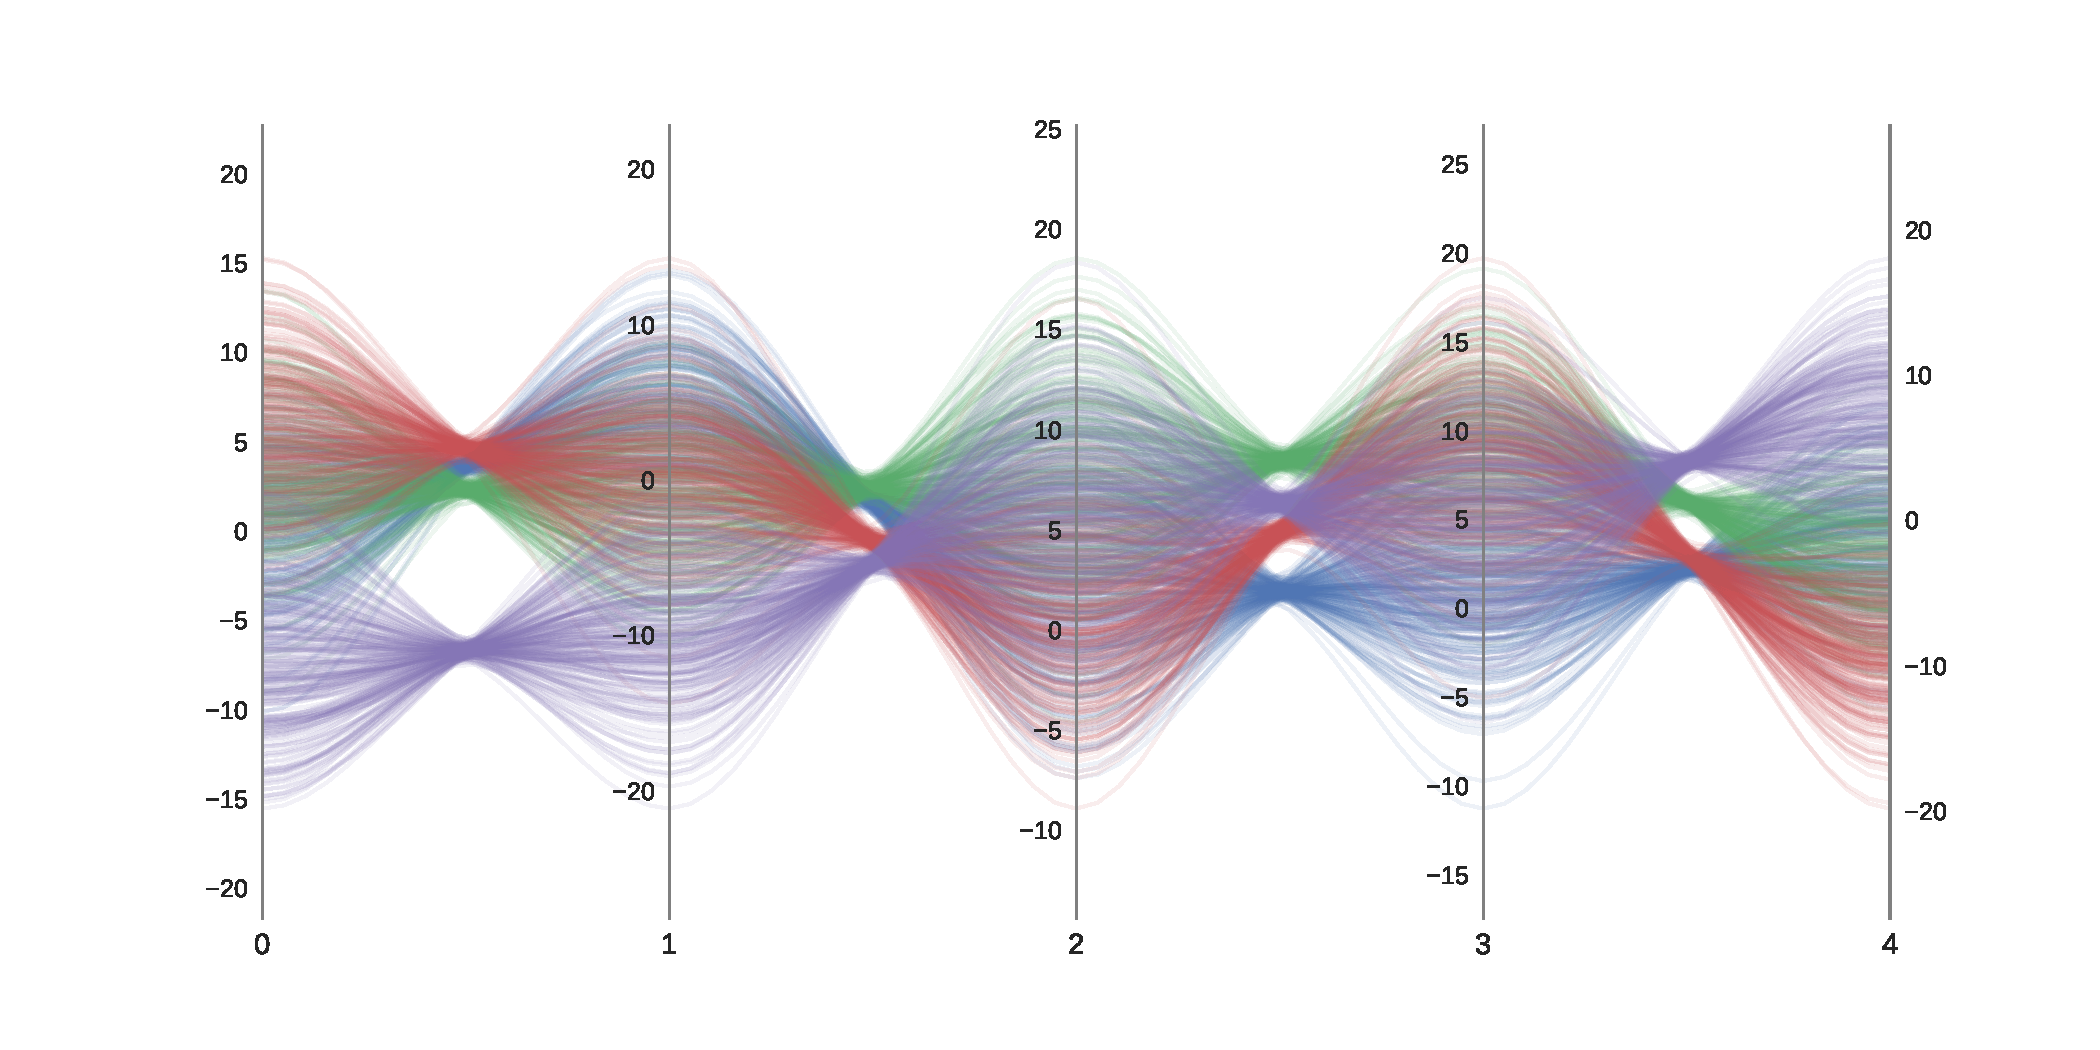
\includegraphics[width=10.5cm]{bad_clustering.pdf}
    \end{figure}
\end{frame}

\begin{frame}{Влияение количества объектов на читаемость}
    \begin{figure}[htb]
        \centering
        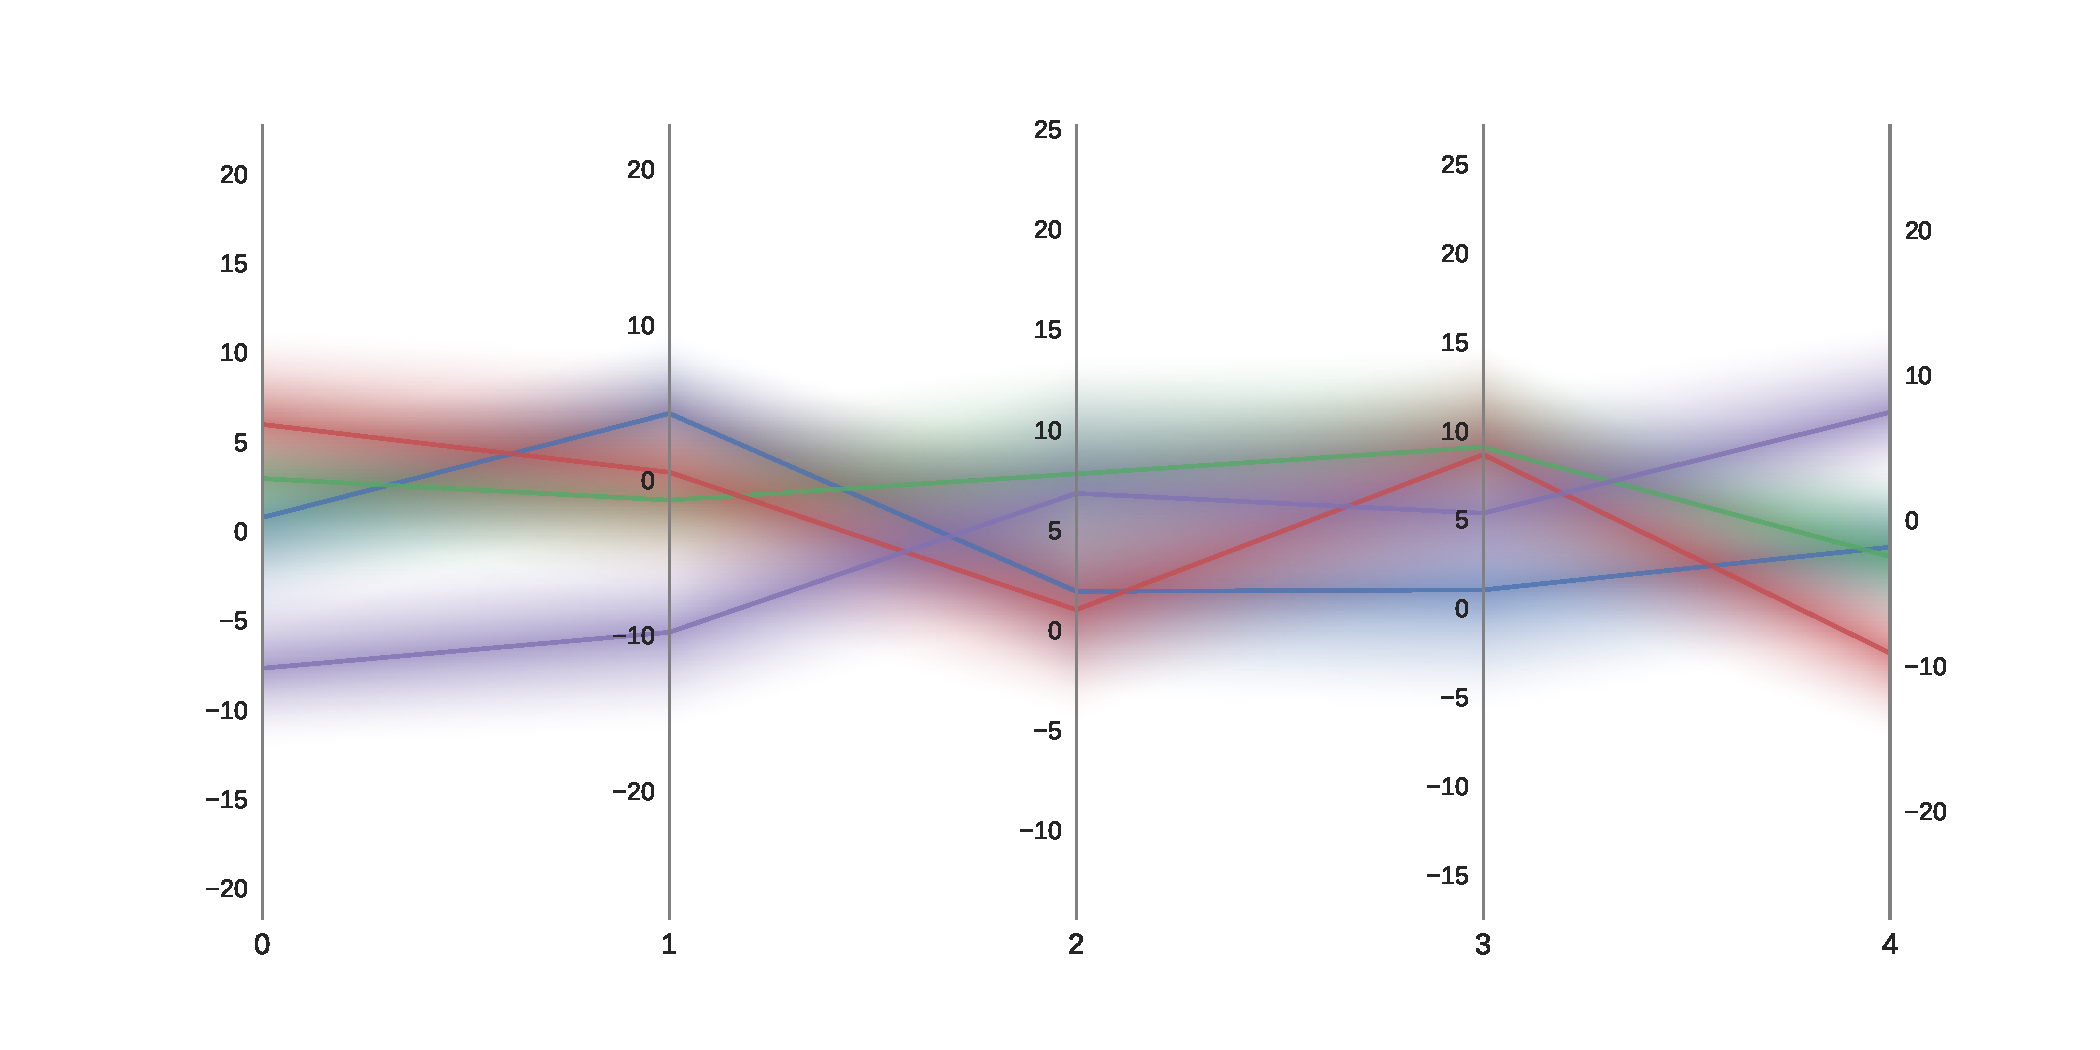
\includegraphics[width=10.5cm]{bad_hierarchical_clustering.pdf}
    \end{figure}
\end{frame}

\begin{frame}{Резюмируя}

    Методы решения проблем:
    \begin{itemize}
        \item Изменение степени прозрачности линий.
        \item Использование гладких линий.
        \item Связывание линий в рамках кластеров.
        \item Отображение лишь части объектов.
        \item \textbf{Изменение порядка и направления осей.}
    \end{itemize}
\end{frame}

\section{Методы выбора порядка}


\begin{frame}{''Правильный'' порядок}
    Формализуем понятие ''правильного'' порядка осей

    \vspace{10pt}

    График хороший, если:
    \begin{itemize}
        \item Линии редко пересекаются между собой
        \item Есть монотонная зависимость между двумя соседними координатами
        \item Направление осей вверх
        \item Слишком шумные ''зависимости'' где-нибудь на последних осях
    \end{itemize}
\end{frame}

\begin{frame}{Корреляция}
    Пусть даны две выборки $X=(x_1, \ldots ,x_n), Y=(y_1,\ldots ,y_n)$.

    \begin{block}{Корреляция Пирсона}
            \centering
            $\rho_{XY} = 
            \frac{\sum\limits_{i=1}^{n}(x_i-\overline x)(y_i-\overline y)}
            {\sqrt{\sum\limits_{i=1}^{n}(x_i-\overline x)^2\sum\limits_{i=1}^{n}(y_i-\overline y)^2}}, 
            \hspace{15px} \left\lvert \rho_{XY} \right\rvert \leq 1$
    \end{block}

    Пусть $R_i$ -- ранг наблюдения $x_i$, $S_i$ -- ранг наблюдения $y_i$

    \begin{block}{Корреляция Спирмена}
        \centering
        $r_{XY} = 
        \frac{\sum\limits_{i=1}^{n}(R_i-\overline R)(S_i-\overline S)}
        {\sqrt{\sum\limits_{i=1}^{n}(R_i-\overline R)^2\sum\limits_{i=1}^{n}(S_i-\overline S)^2}},
        \hspace{15px} \left\lvert r_{XY} \right\rvert \leq 1$
    \end{block}
    $\rho_{XY} = 0$, $r_{XY} = 1$, где $X=Y^2$ и $X$ симметрично распределена относительно нуля.

\end{frame}

\begin{frame}{Минимизируемый функционал}
    Пусть $\pi = (\pi_1, \ldots , \pi_n)$ перестановка множества $\{1,\ldots, n\}$, где $n$ размерность пространства.

    Мы хотим максимизировать такой функционал: 
    $$\sum\limits_{i=1}^{n-1}|r_{X^{\pi_i}X^{\pi_{i+1}}}| \rightarrow \min\limits_\pi$$
    где $r_{X^iX^j}$ -- Корреляция Спирмена между  $i$ координатой и $j$ координатой.
    
    \vspace{10pt}

\end{frame}


\begin{frame}{}

    \begin{block}{Задача о самом длинном пути}
    Это задача поиска простого пути максимальной длины в заданном графе.
    Является NP-трудной и не может быть решена за 
    полиномиальное время для произвольных графов.
    \end{block}

    \vspace{10px}

    Пусть $X=(x_1,\ldots,x_n)$ -- выборка, где $x_i\in \mathbb{R}^n$. 

    \vspace{10px}

    Построим связный граф $G(V,E)$, где каждая вершина $u^i \in V$ соответствует
    i-ой координатe (i-ой оси на графике), а каждому ребру $\{u^i,u^j\} \in E$ сопоставим вес равный $|r_{X^iX^j}|$.

\end{frame}

\begin{frame}{}

    \begin{itemize}
        \item Простейшим перебором задача решается за $O(n!)$
        \item Можно свести к задаче коммивояжера.
        \item С помощью методов динамического программирования можно улучшить асимптотику решения.
    \end{itemize}

    \vspace{10px}

    \begin{tabular}{cc}
        \centering
        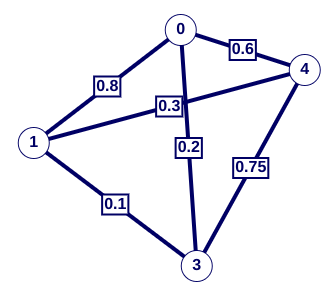
\includegraphics[width=5cm]{graph_example_1.png} &
        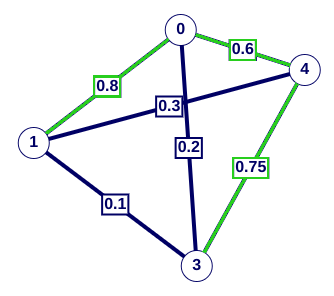
\includegraphics[width=5cm]{graph_example_2.png}   \\
    \end{tabular}
\end{frame}

\begin{frame}{Пример использования}
    Классический вид

    \begin{figure}[htb]
        \centering
        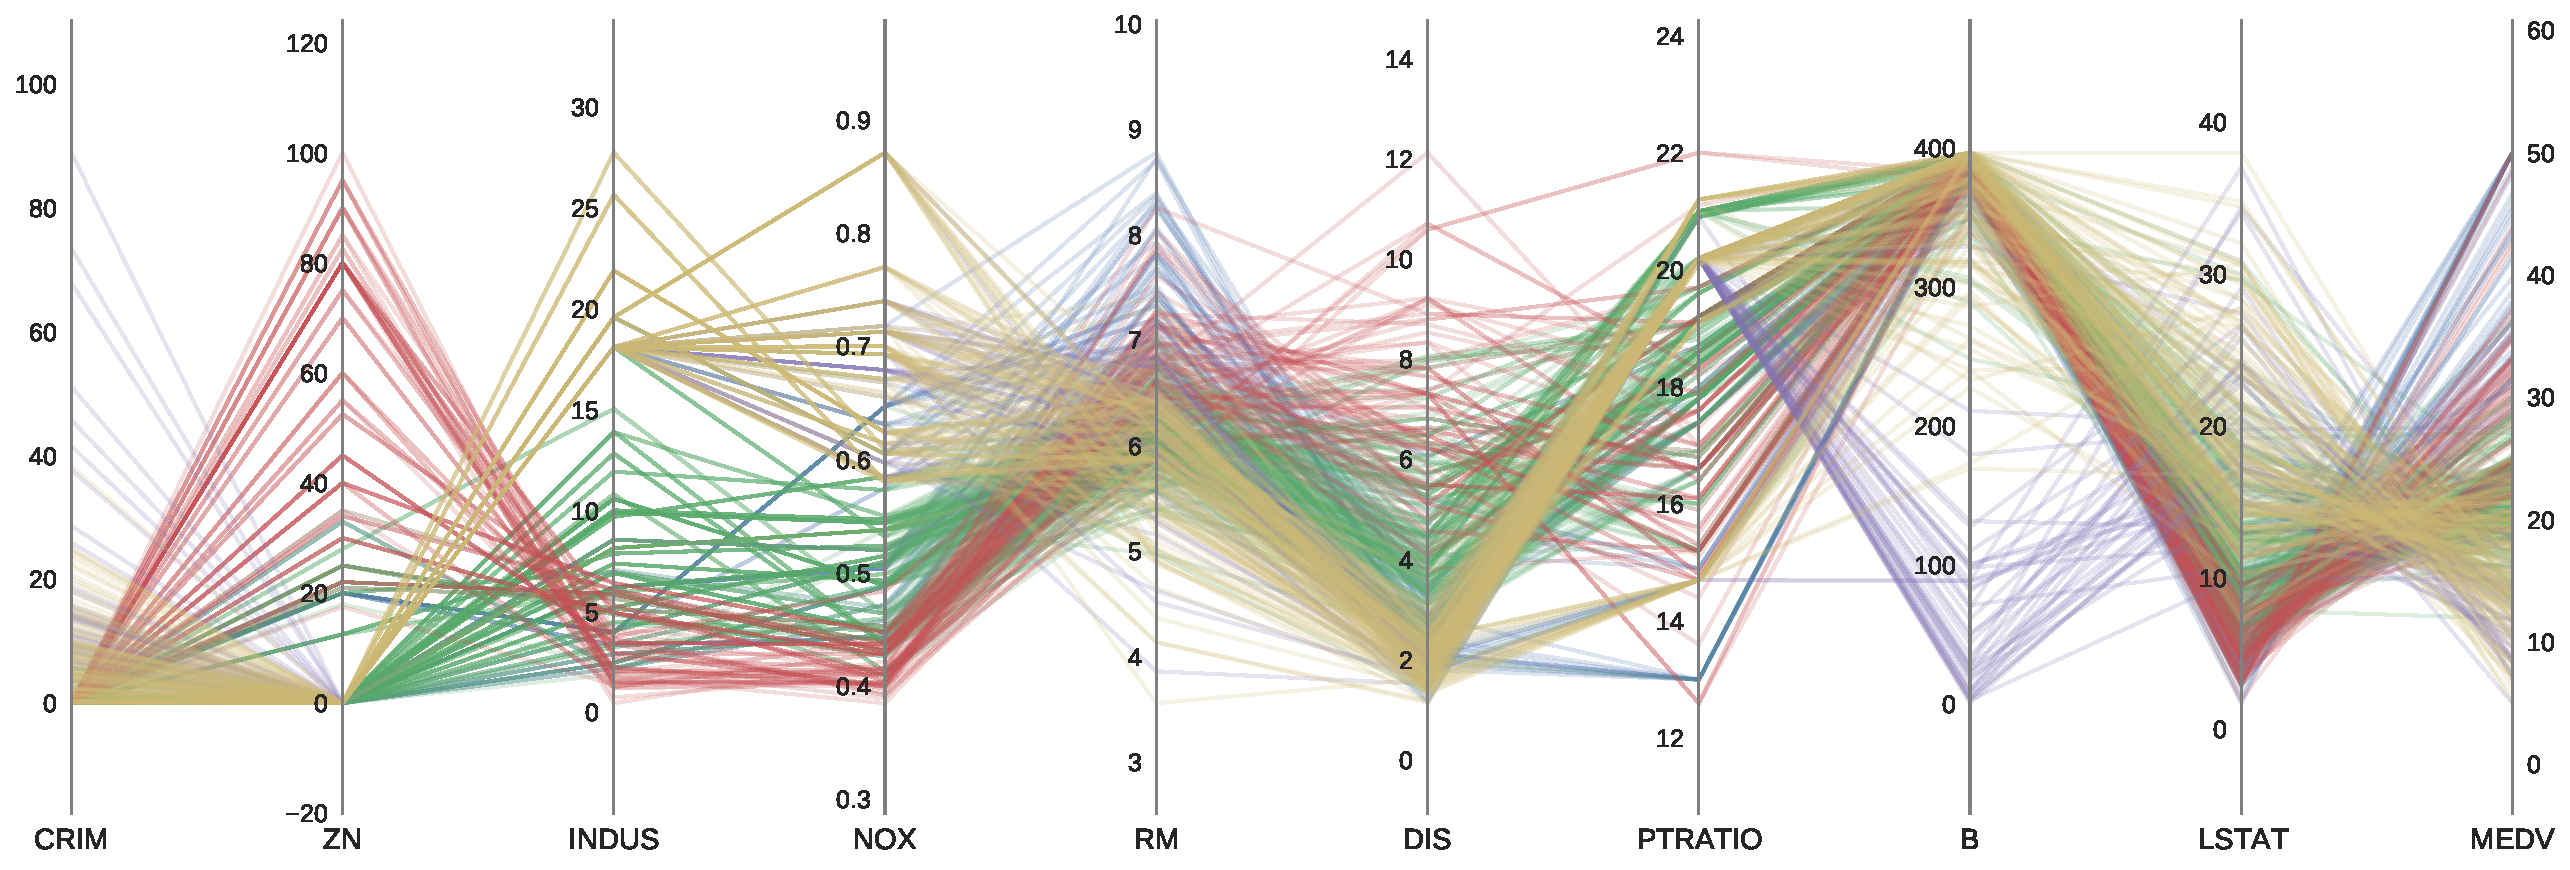
\includegraphics[width=11cm]{housing_example_1.pdf}
    \end{figure}

    \textit{Датасет boston housing}
    
    \textit{Предварительно проведена кластеризация KMeans}
\end{frame}

\begin{frame}{Пример использования}
    Со сплайнами и связыванием

    \begin{figure}[htb]
        \centering
        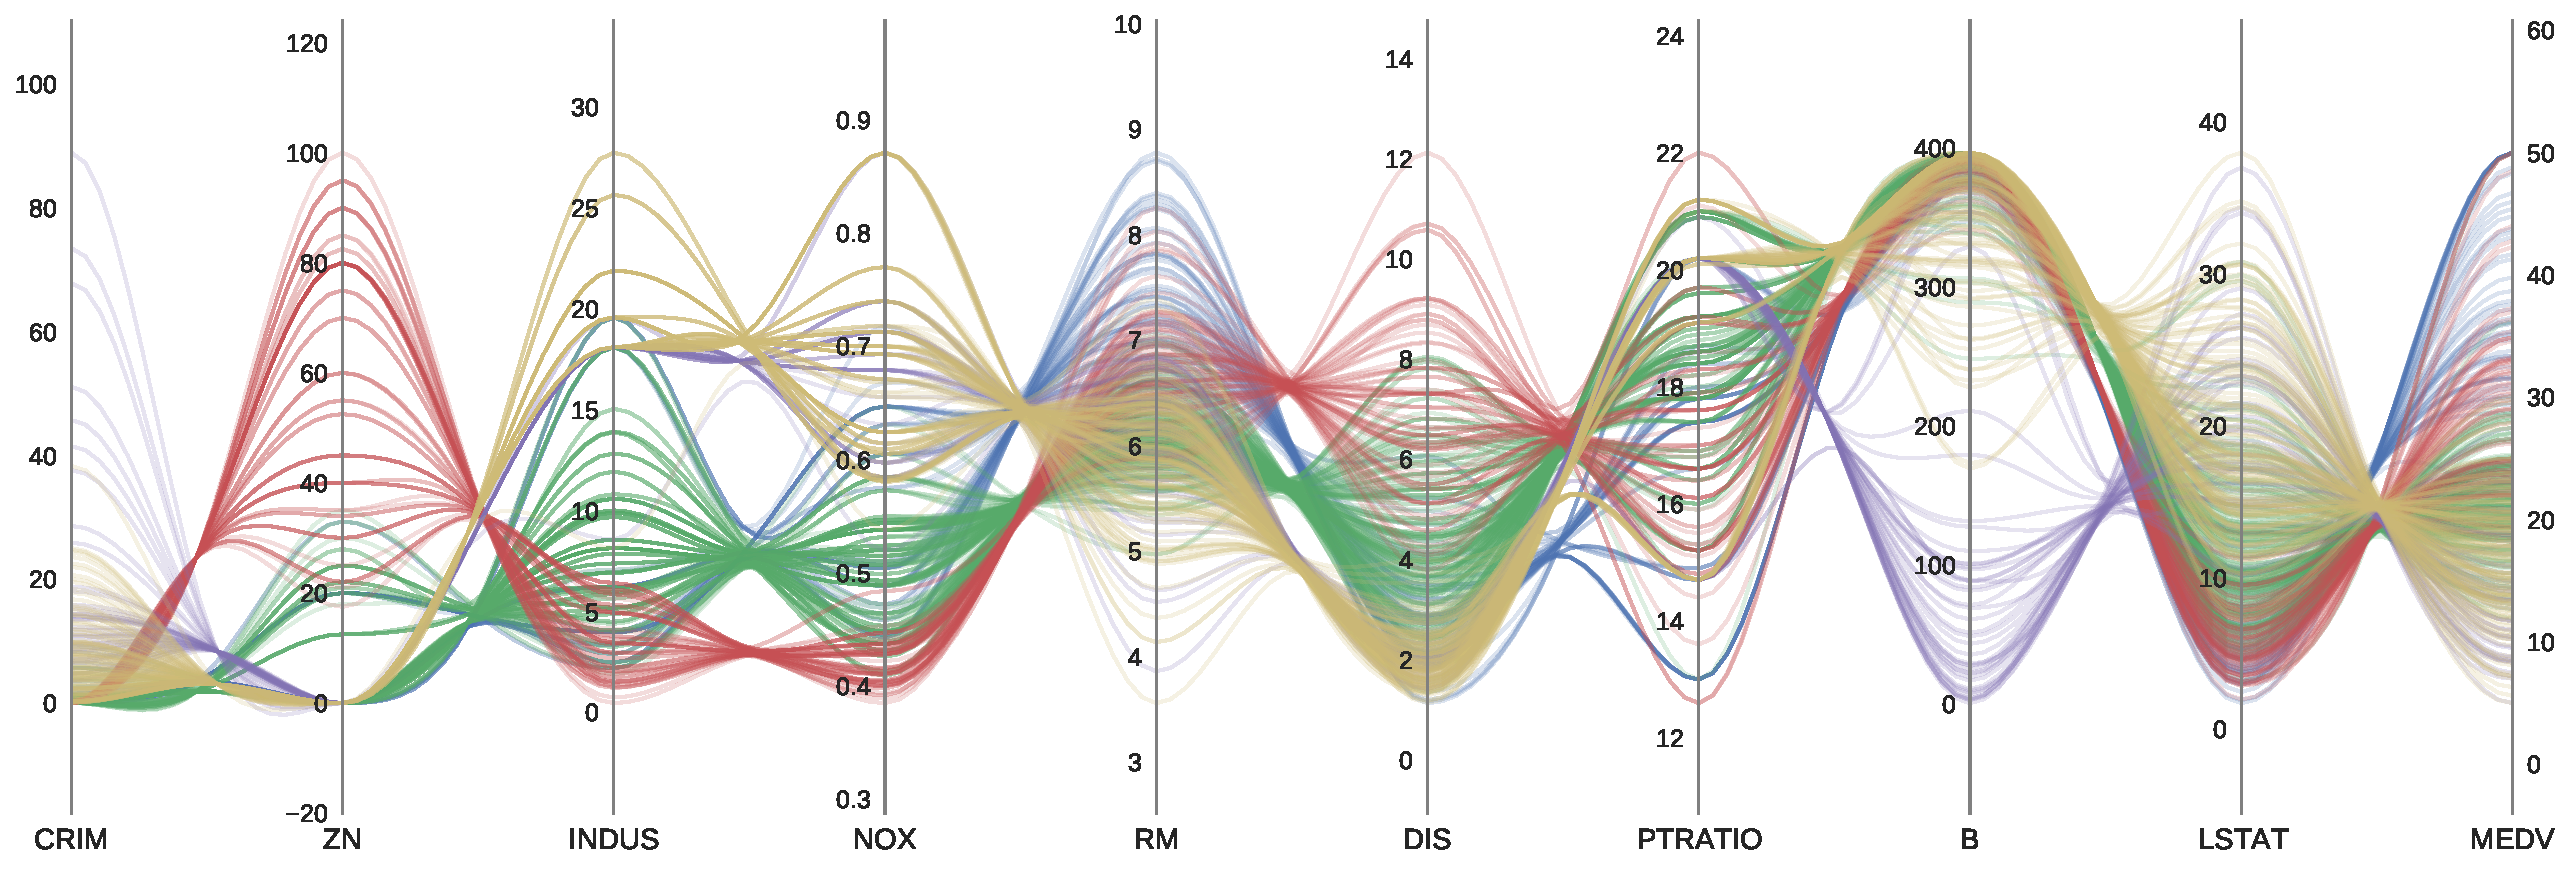
\includegraphics[width=11cm]{housing_example_2.pdf}
    \end{figure}
\end{frame}

\begin{frame}{Пример использования}
    С агрегацией

    \begin{figure}[htb]
        \centering
        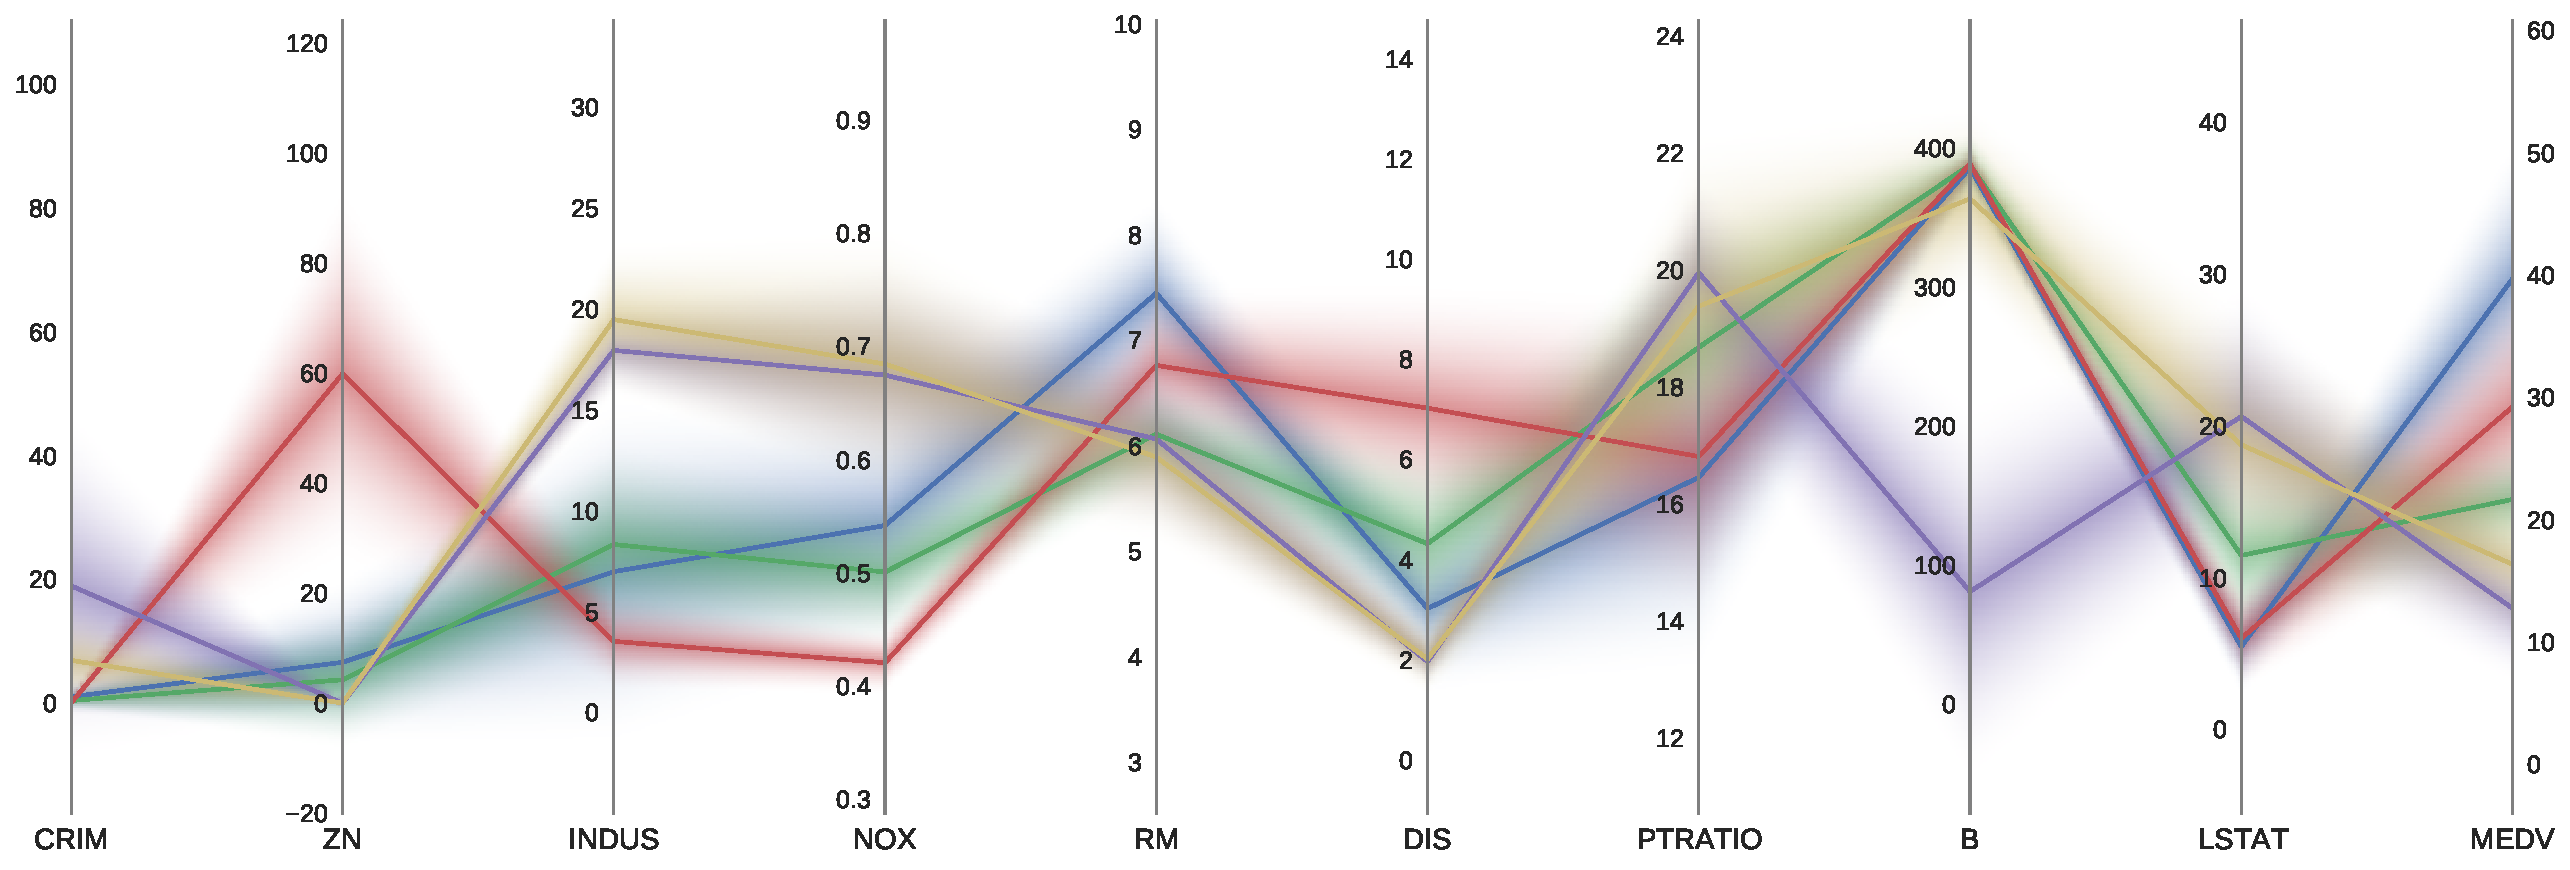
\includegraphics[width=11cm]{housing_example_3.pdf}
    \end{figure}
\end{frame}

\begin{frame}{Пример использования}
    Сплайны + связывание + оптимальный порядок осей

    \begin{figure}[htb]
        \centering
        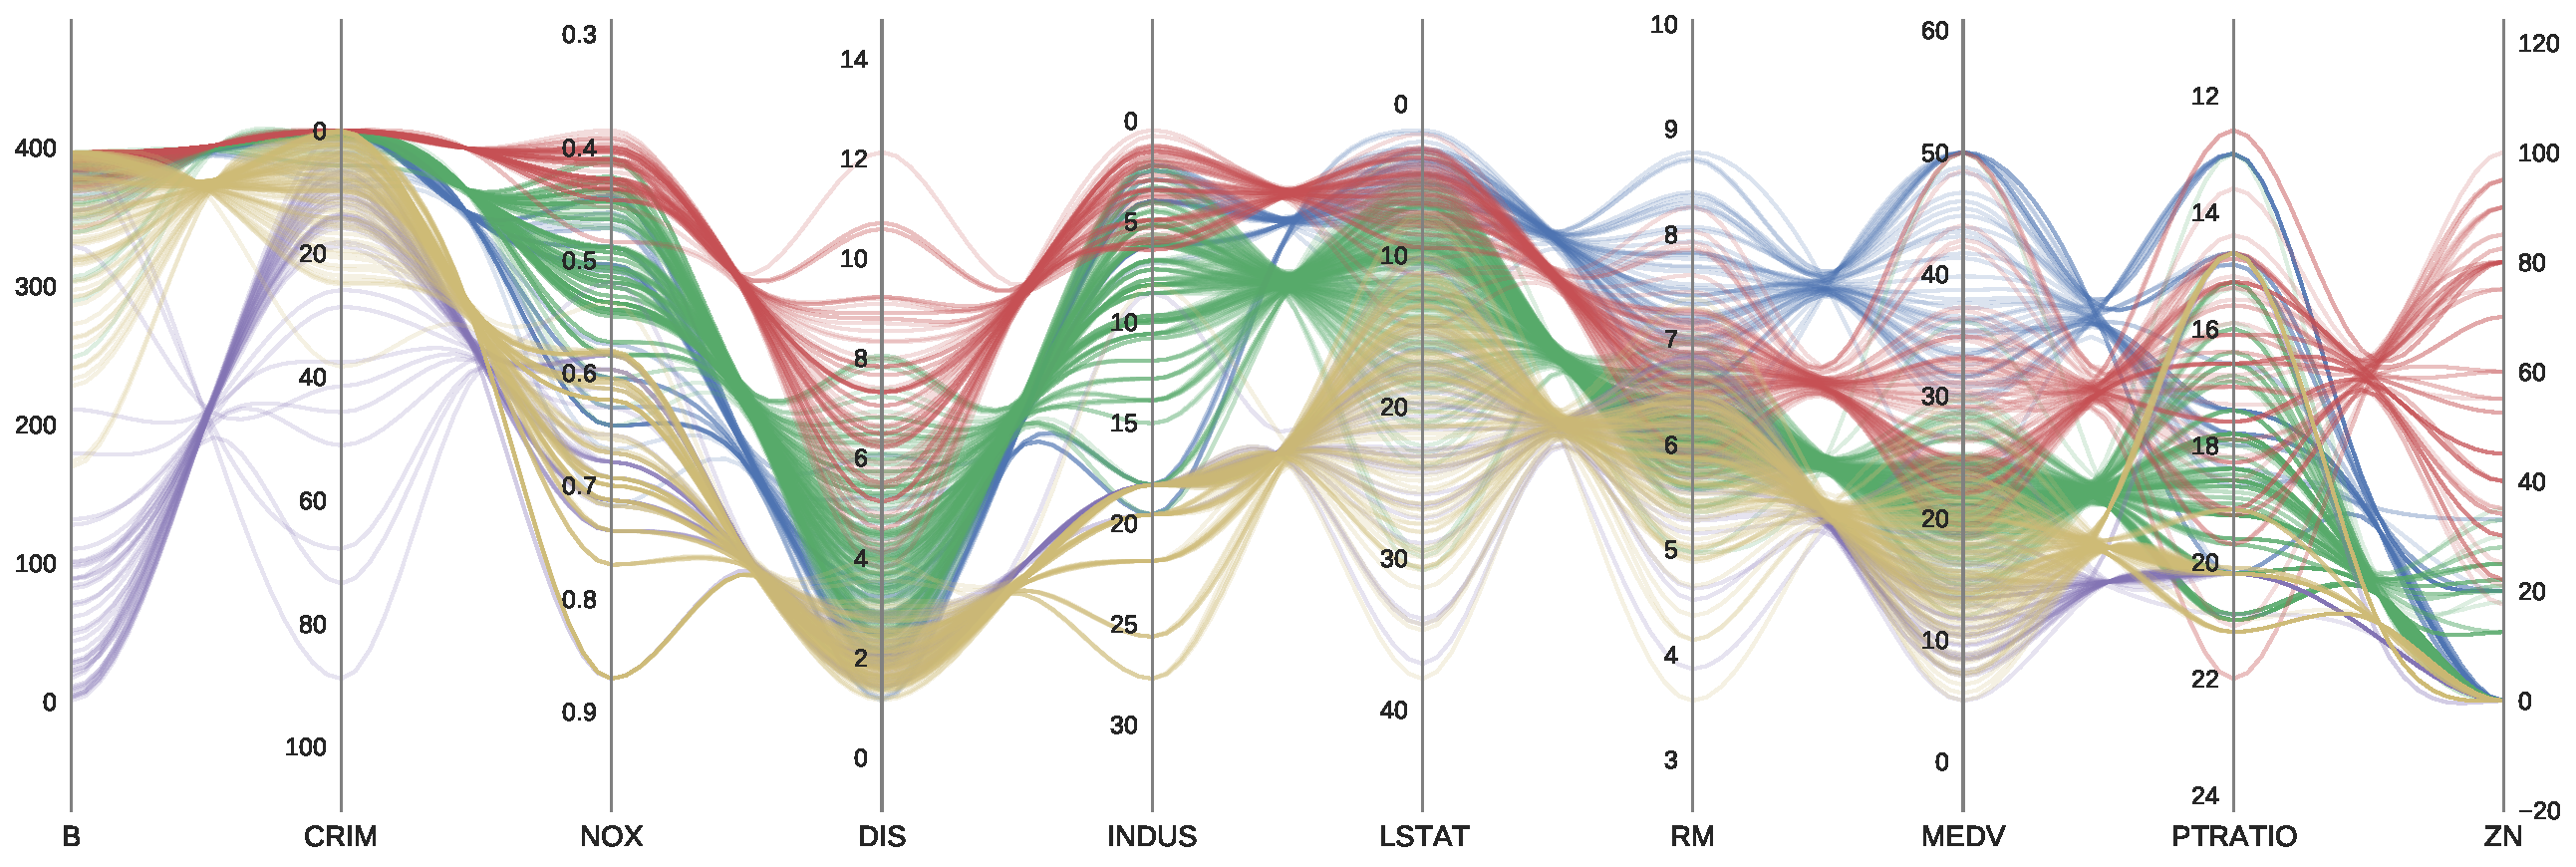
\includegraphics[width=11cm]{housing_example_4.pdf}
    \end{figure}
\end{frame}

\begin{frame}{Пример использования}
    Агрегация + оптимальный порядок осей

    \begin{figure}[htb]
        \centering
        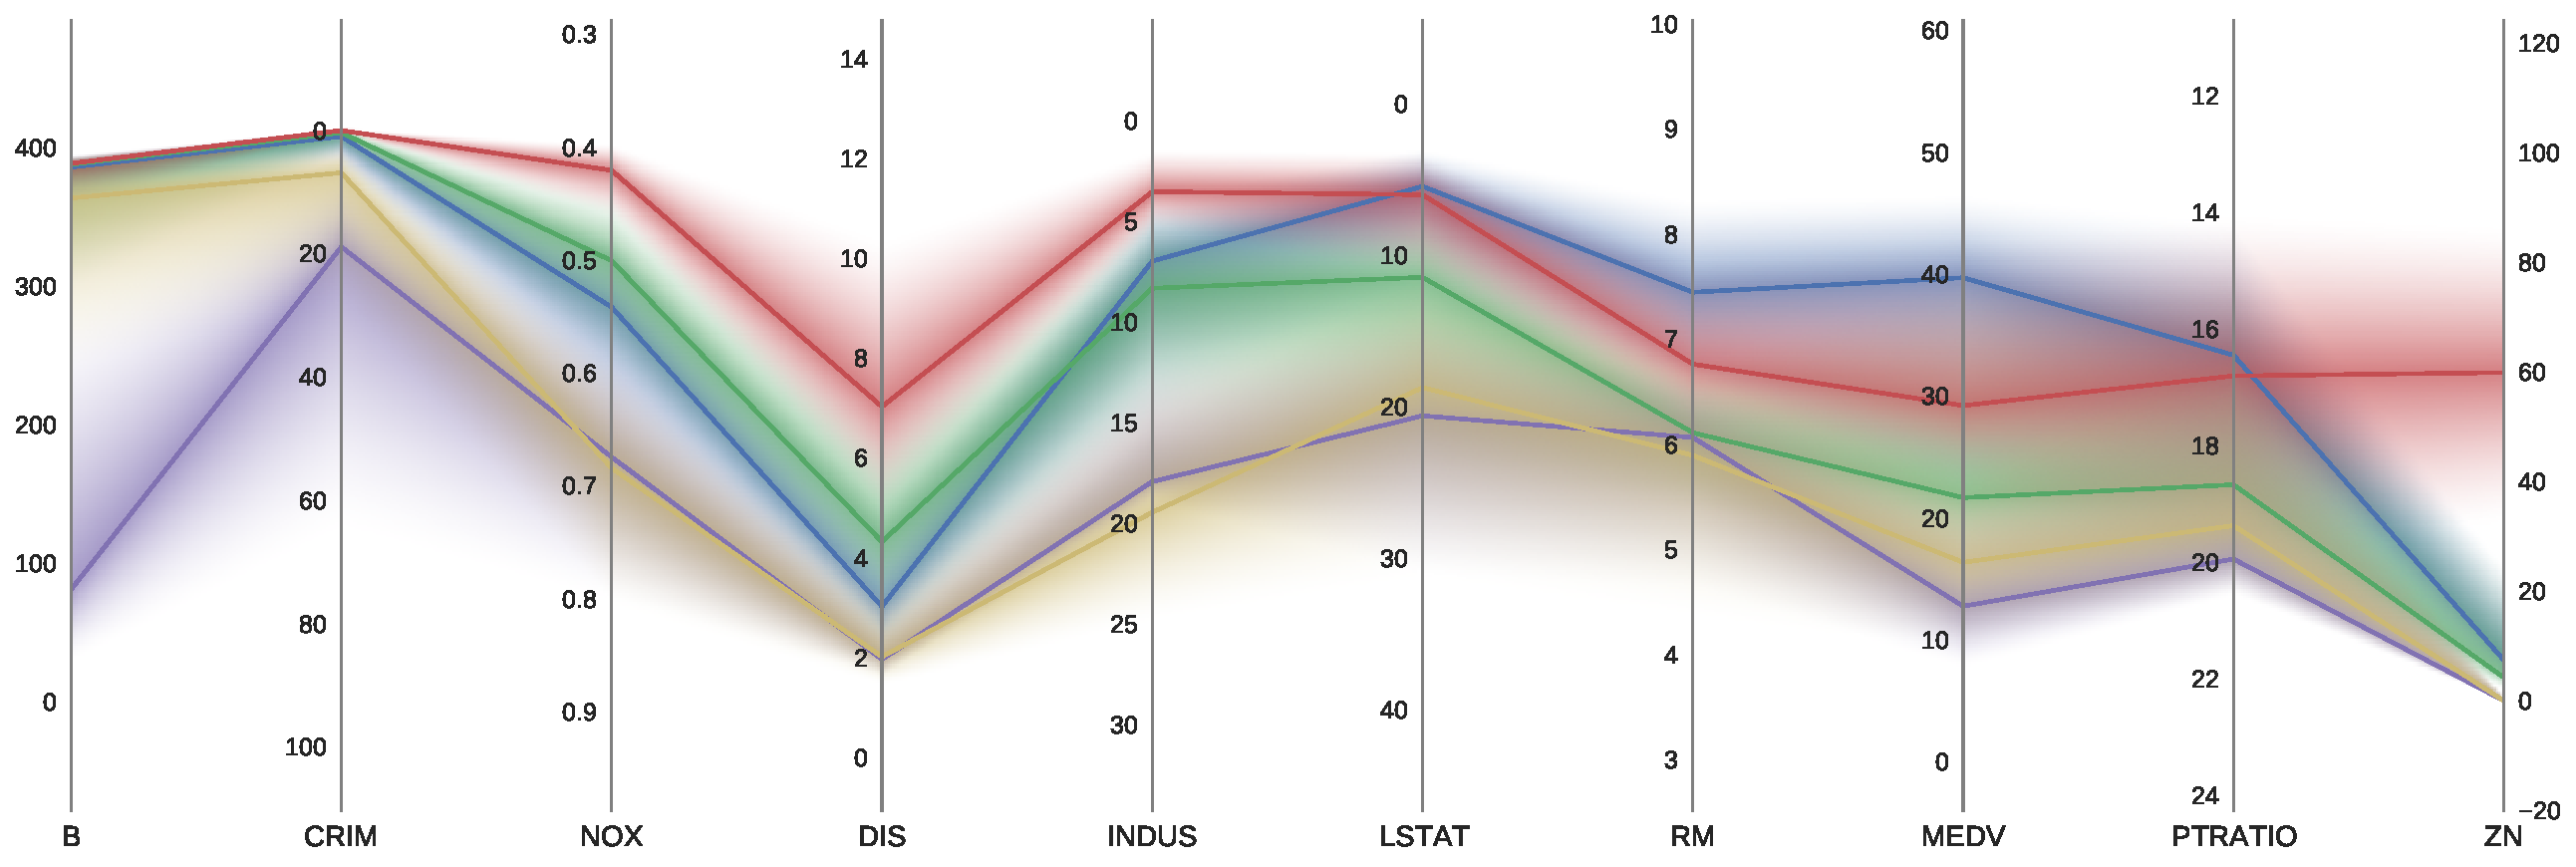
\includegraphics[width=11cm]{housing_example_5.pdf}
    \end{figure}

\end{frame}

\section{О библиотеке}

\begin{frame}{Обзор текущих средств}

    \begin{itemize}
        \item На Python есть простейшая реализация лишь в библиотеке pandas!
        \item ELKI, GGobi, Mondrian, Orange и ROOT.
        \item Parcoords.js интерактивная библиотека на JavaScript.
    \end{itemize}

\end{frame}

\begin{frame}{Цели}
    \begin{itemize}
        \item Дать возможность исследователям ''безболезненно'' использовать график
              в параллельных осях.
        \item Построение красивых и информативных графиков из ''коробки''.
        \item Реализация всевозможных видов данных графиков.
    \end{itemize}
\end{frame}

\begin{frame}{Технические подробности}
    \begin{itemize}
        \item Статические графики.
        \item Библиотека пишется на языке Python на базе matplotilb.
        \item Простой высокоуровневый интерфейс. Как и в библиотеке seaborn методы могут принимать pandas.DataFrame,
              обычные numpy массивы или списки -- для всего единый интерфейс.
    \end{itemize}
\end{frame}

\begin{frame}{Возможности}
    Построение классических графиков в параллельных осях
        \begin{itemize}
            \item Возможность рисовать гладкие линии.
            \item Возможность ''связывания'' линий кластеров.
            \item Возможность ''связывания'' линий на основе близости.
        \end{itemize}

    Построение иерархических графиков
        \begin{itemize}
            \item Отрисовка полупрозрачного градиента.
            \item Работа с иерархическими кластерами.
            \item Изображение распределения с помощью градиента.
        \end{itemize}

    Дополнительные возможности
    \begin{itemize}
        \item выделение подмножества линий в  диапазоне значений одной из осей.
        \item нахождение оптимального расположения осей.
        \item создание иерархических кластеров на основе входящей выборки.
    \end{itemize}
\end{frame}

\begin{frame}{Итоги}
   
    \begin{figure}[htb]
        \centering
        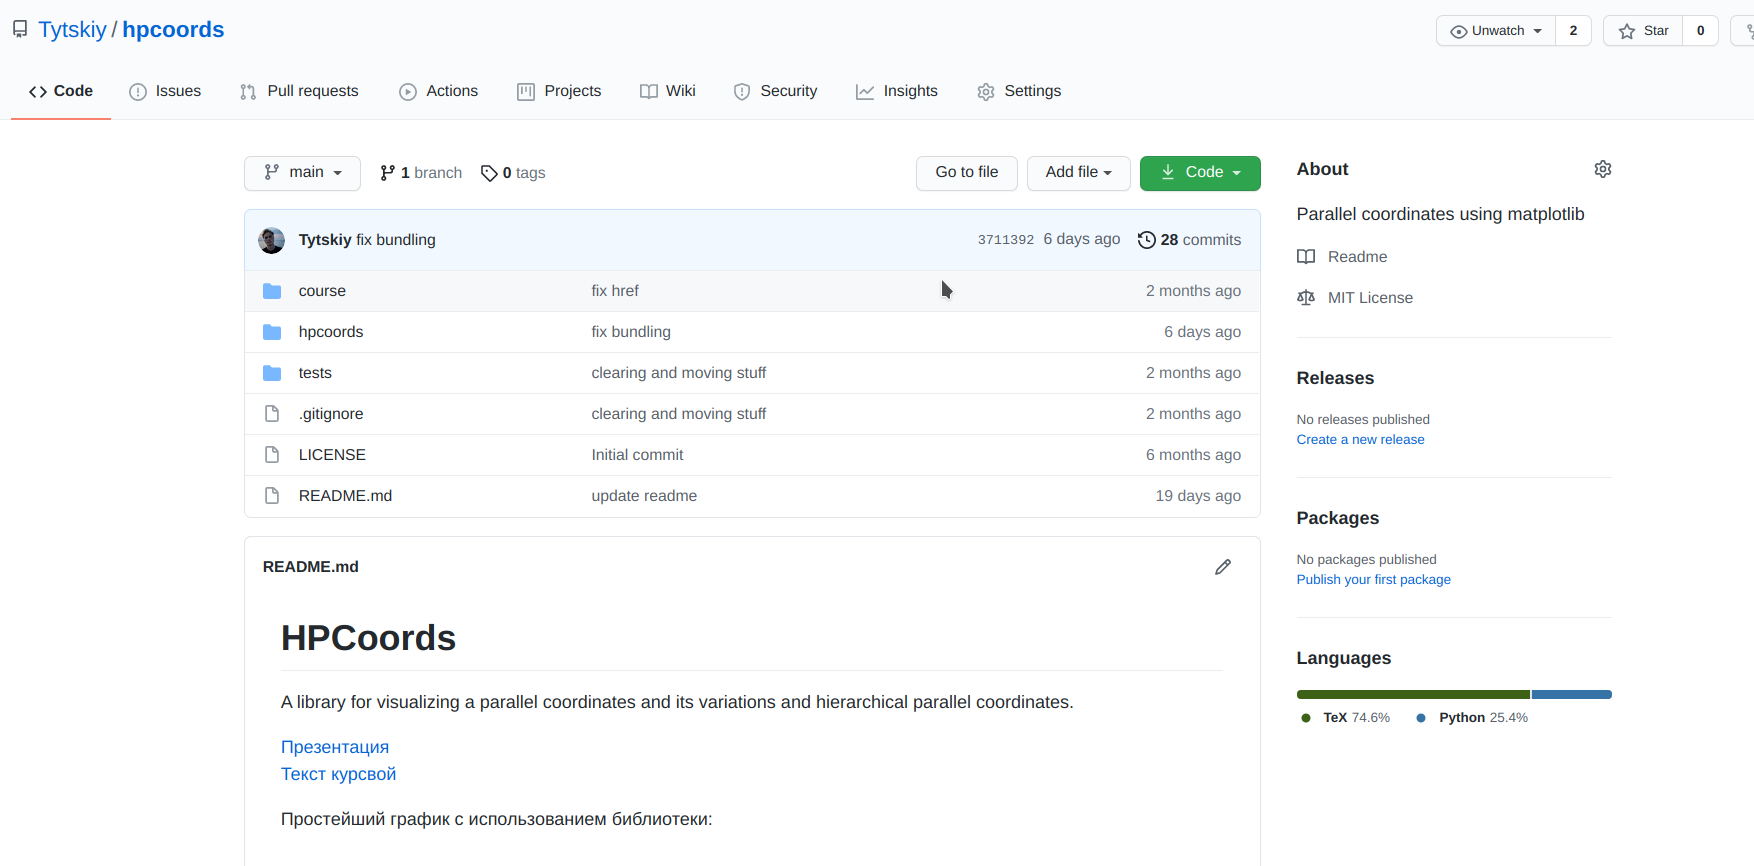
\includegraphics[height=5cm]{github_screen.png}
    \end{figure}
    \begin{itemize}
        \item Реализовано API для визуализации всех основных графиков.
        \item Совсем скоро добавлю библиотеку в пакетные менеджеры.
        \item Работаю над реализацией дополнительных возможностей
    \end{itemize}
    
\end{frame}


\begin{frame}{Итоги}
   
    \begin{itemize}
        \item Написана библиотека для визуализации графика в параллельных осях.
        \item Предложены новые способы улучшения читаемости графика.
        \item График в параллельных осях очень мощный инструмент визуализации.
    \end{itemize}
    
\end{frame}


\begin{frame}{Ссылки}
    \textit{https://github.com/Tytskiy/hpcoords}

    \vspace{10pt}

    \begin{thebibliography}{9}
        \bibitem{inselberg} 
        Inselberg A. 
        \textit{The plane with parallel coordinates}. 
        The visual computer. 1985. – Т. 1. – №. 2. – С. 69-91.
        
        \bibitem{einstein} 
        Fua Y. H., Ward M. O., Rundensteiner E. A. 
        \textit{Hierarchical parallel coordinates for exploration of large datasets.}.
        IEEE, 1999. – С. 43-508.
        
        \bibitem{yang} 
        KYang, Jing; Peng, Wei; Ward, Matthew O.; Rundensteiner, Elke A.
        \textit{Interactive Hierarchical Dimension Ordering 
        Spacing and Filtering for Exploration of High Dimensional Datasets.}
        IEEE Symposium on Information Visualization, 2003. INFOVIS 2003: 3–4.
        \end{thebibliography}

    

     

    
    
\end{frame}


\end{document}